% tADRguide.tex
% v1.0 released January 2013

\documentclass{tADR2e}

% The following packages can be found on http:\\www.ctan.org
\usepackage{caption}
\usepackage{color}
\usepackage{graphicx} % for pdf, bitmapped graphics files
%\usepackage{epsfig} % for postscript graphics files
\usepackage{mathptmx} % assumes new font selection scheme installed
\usepackage{amsmath} % assumes amsmath package installed
\usepackage{amssymb}  % assumes amsmath package installed
\usepackage{mathrsfs}
\DeclareMathOperator*{\argmin}{argmin}
\usepackage{algorithm}
\usepackage{algpseudocode}  %\usepackage[noend]{algpseudocode}
\algtext*{EndWhile}% Remove "end while" text
\algtext*{EndIf}% Remove "end if" text
\usepackage{booktabs}
\usepackage{multirow}
\usepackage{proof}
\newtheorem{property}{Property}
\usepackage[numbers]{natbib}
\algnewcommand\algorithmicinput{\textbf{Input:}}
\algnewcommand\INPUT{\item[\algorithmicinput]}
\algnewcommand\algorithmicoutput{\textbf{Output:}}
\algnewcommand\OUTPUT{\item[\algorithmicoutput]}
\makeatletter
\makeatother
\usepackage{hyperref}
\usepackage{xcolor}
\hypersetup{
    colorlinks,
    linkcolor={red!80!black},
    citecolor={blue!80!black},
    urlcolor={blue!80!black}
}
\usepackage{minibox}
\usepackage{array}
\newcolumntype{L}[1]{>{\raggedright\let\newline\\\arraybackslash\hspace{0pt}}p{#1}}
\newcolumntype{C}[1]{>{\centering\let\newline\\\arraybackslash\hspace{0pt}}p{#1}}
\newcolumntype{R}[1]{>{\raggedleft\let\newline\\\arraybackslash\hspace{0pt}}p{#1}}

% Math shortcuts :
\newcommand\real{\mathbb{R}}
\newcommand\p{\mathbf{p}}
\newcommand\gT{\tilde{g}^T}
\newcommand\g{\tilde{g}}
\newcommand\CS{\mathcal{C}}
\newcommand\dimCS{n_\mathbf{C}}
\newcommand\body{{\cal B}}
\newcommand\Sone{\mathbf{S}^1}
\newcommand\Sthree{\mathbf{S}^3}
\newcommand\conf{\mathbf{q}}
\newcommand\xx{\mathbf{x}} % \x already defined in the class
\newcommand\cost{C}
\newcommand\weight{W}
\newcommand\translation{\mathbf{t}}
%\newcommand\tcolli{t_{coll\ i}}
\newcommand\tcolli{\kappa_i}
\newcommand\po{\mathbf{P}}
\newcommand\Jf{\Phi}
\newcommand\kernel{\mbox{Ker }}
\newcommand\U{\mathbf{u}}
\newcommand\rotation{R}
\newcommand\traj{\Gamma}
\newcommand\velocity{\mathbf{v}}
\newcommand\todo{\textcolor{red}{NOT FINISHED}}
%%%%%%%%%%%%%%%%%%%%%%%%%%%%%%%%%%%%%%%%%%%%%%%%%%%%%%%%%%%%%%%%%%%%%%%%%%%%%%%%
\begin{document}
\graphicspath{{images/}}



\title{\textcolor{blue}{A gradient-based optimization method for motion planning}$^{1}$}

\author{Myl\`{e}ne Campana$^{\ast}$ \thanks{$^\ast$Corresponding author. Email: \href{mailto:mcampana@laas.fr}{mcampana@laas.fr}}, Florent Lamiraux and Jean-Paul Laumond
\\\vspace{6pt}
{\em{LAAS-CNRS, 7 av. Colonel Roche, 31400 Toulouse, FRANCE}}
}
\maketitle



\begin{abstract}
Most algorithms in probabilistic sampling-based path planning compute 
collision-free paths made of straight line segments lying in the configuration 
space. Due
to the randomness of sampling, the paths make detours that need to be optimized.
The contribution of this paper is to propose a basic gradient-based (GB) algorithm 
that transforms a polygonal collision-free path into a shorter one.
While requiring only collision 
checking, and not any time-consuming obstacle distance computation nor geometry 
simplification, we constrain only part of the configuration variables 
that may cause a collision, and not entire configurations. Thus parasite motions that 
are not useful for the problem resolution are reduced without any 
assumption.
Experimental results include navigation and manipulation tasks, 
e.g. a manipulator arm filling boxes and a PR2 robot working in a kitchen 
environment. Comparisons with a random shortcut optimizer and a partial 
shortcut have also been studied.

% one line version:
%Most algorithms in probabilistic sampling-based path planning compute collision-free paths made of straight line segments lying in the configuration space. Due to the randomness of sampling, the paths make detours that need to be optimized. The contribution of this paper is to propose a basic gradient-based (GB) algorithm that transforms a polygonal collision-free path into a shorter one. While requiring only collision checking, and not any time-consuming obstacle distance computation nor geometry simplification, we constrain only part of the configuration variables that may cause a collision, and not entire configurations. Thus parasite motions that are not useful for the problem resolution are reduced without any assumption. Experimental results include navigation and manipulation tasks, e.g. a manipulator arm filling boxes and a PR2 robot working in a kitchen environment. Comparisons with a random shortcut optimizer and a partial shortcut have also been studied.

% few parameter tuning REMOVED

\medskip

\begin{keywords}path optimization; motion planning; robotics
\end{keywords}\medskip

\end{abstract}


\section{Introduction}
Motion planning for systems in cluttered environments has been addressed for more
than thirty years~\cite{ref-motionplan}. 
To explore the connected components of collision-free configuration spaces, pioneering 
contributions in the 90’s introduced certain levels of random searches, i.e. random walks in~\cite{potentielBarraquandLatombe}, random sampling in 
~\cite{KavrakiLatombePRM} and~\cite{LaValleKuffnerRRT}. Today most motion planners are inspired by these seminal approaches.
The main issue using these techniques is that the computed path makes unnecessary 
detours and needs to be post-processed before being executed by a virtual or real 
robot. Alternative strategies exist however.
\begin{itemize}
\item Planning by path-optimization~\cite{itomp2012},~\cite{voronoiOMP} where
obstacle avoidance is handled by constraints or cost using computation of the
nearest obstacle distance. Most of these planners are using non-linear
optimization~\cite{BettsNonlinopt} under constraints. Such planners provide close-to-optimality paths and have smaller time computation
for easy problems, but they are mostly unable to solve narrow passage issues.
 
\item Optimal random sampling~\cite{KaramanPRMstarRRTstar} are also close to an
optimal solution, but computation time is significantly higher than classical
approaches.
\end{itemize}

\textcolor{blue}{Optimization is always regarding to one or several criteria. The most common in motion planning are the path length, which penalize detours, the obstacle clearance for safety and the execution time, which is influenced by the number of via points, introducing velocity discontinuities. One can also mention the minimization of the acceleration or jerk peaks to safely play the motion on a robot.}

In this paper, we propose a method aimed at shortening path length after a path
planning step. Note that we do not address path planning, but that we take the
result of a probabilistic motion planner as the input to our path optimization 
method.

\begin{figure}
	\centering
	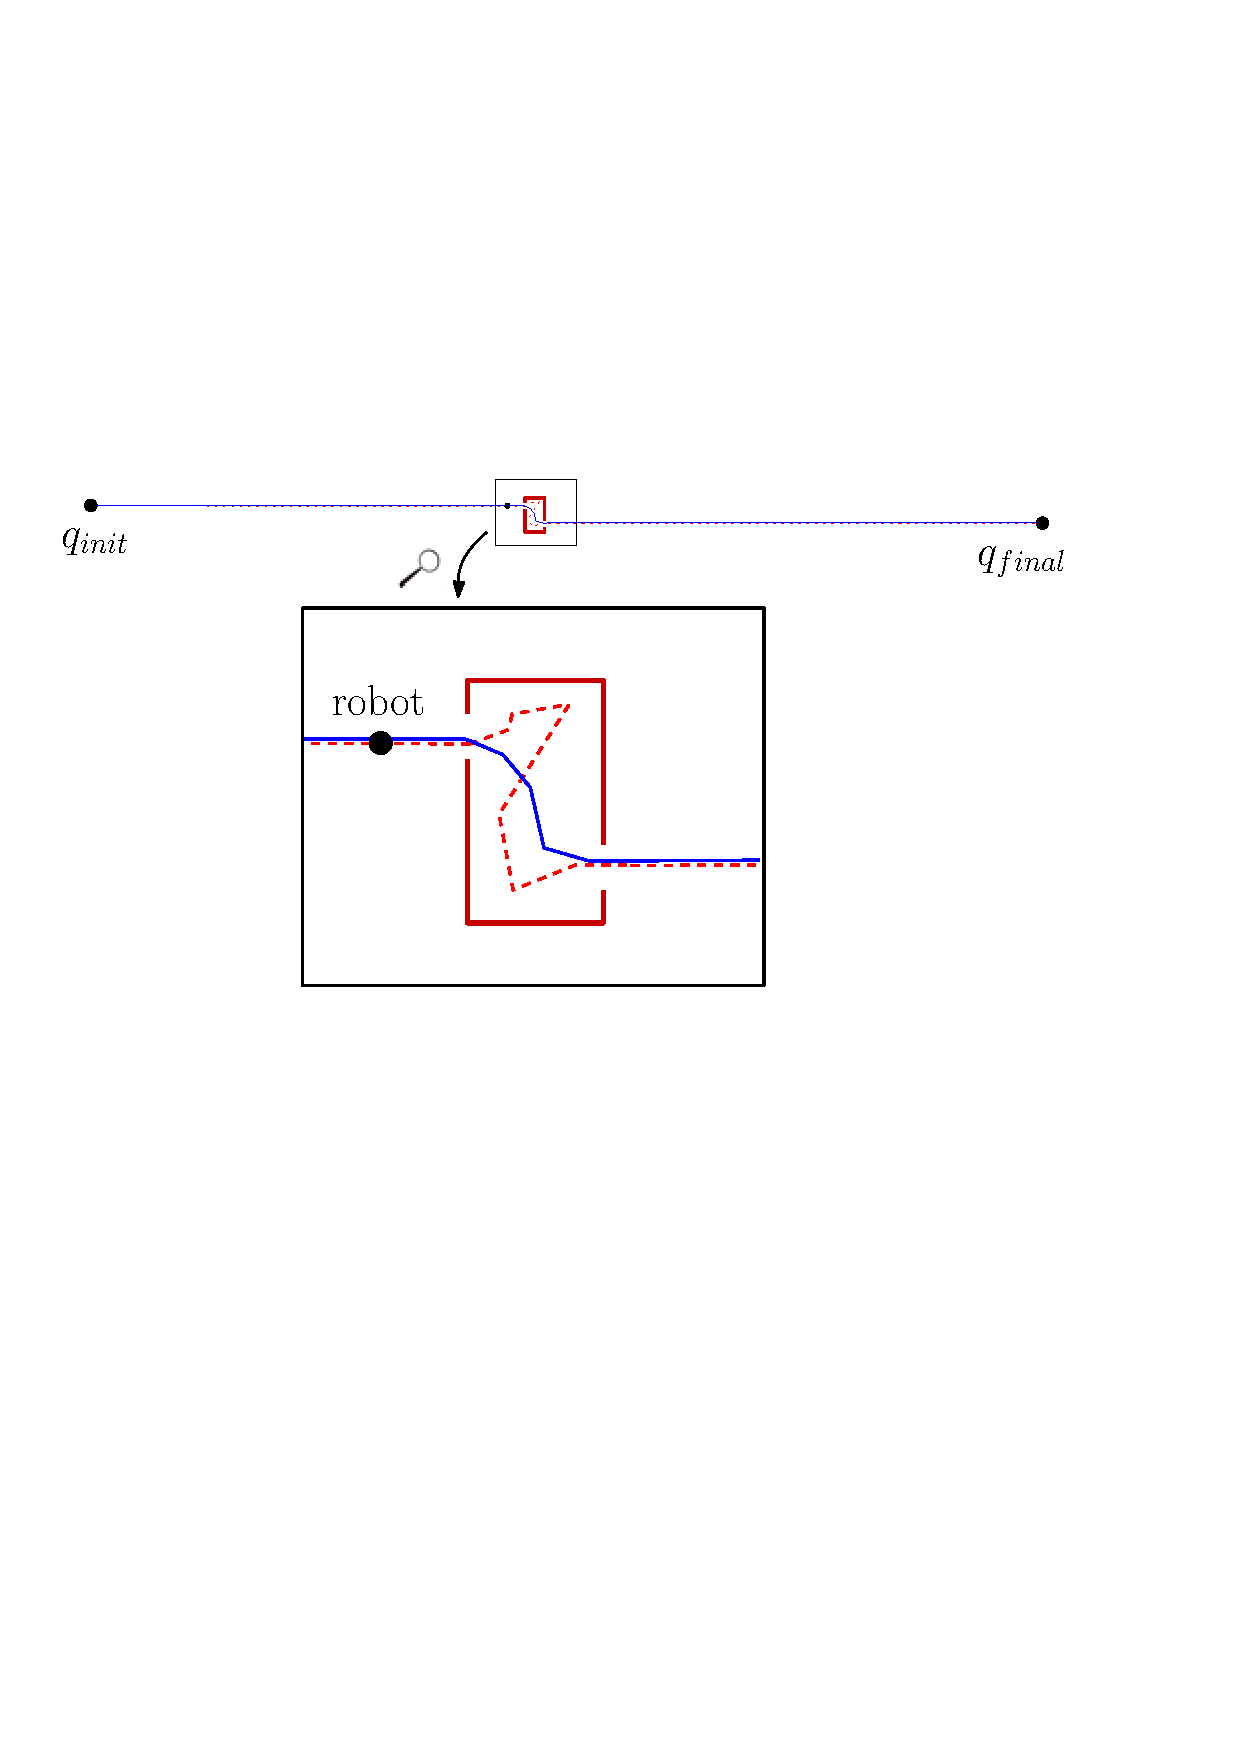
\includegraphics[width=10cm]{local_box_optim2.pdf}
	\caption{Case of a long initial path from $\conf_{init}$ to $\conf_{final}$ (above) containing a small part 
	that can 
	be optimized (below). Random shortcut is unlikely to optimize the initial 
	dashed part containing detours in the box, whereas our method 
	succeeds (in blue). This type of issue is common in navigation problems, in 
	environments with long corridors.}
	\label{local_box_optim}
\end{figure}

For this shortening purpose, random shortcut (RS) methods are
still very 
popular~\cite{Sekhavat-Svestka1998,GeraertsIJRR07,HauserFastSmooth}. 
However, RS requires fine 
tuning of the termination condition and is no efficient for long 
trajectories where only a minor part needs to be optimized, 
as in \textcolor{blue}{Figure~\ref{local_box_optim}}.
Figure~\ref{decoupled_DOF_optimization} presents another situation where RS 
will always fail to optimize the initial path, since it cannot decouple the 
robot degrees of freedom (DOF) on which the optimization occurs. This problem is 
addressed by our method.
\textcolor{blue}{Processing a path 
pruning~\cite{GeraertsIJRR07}, in order to remove redundant nodes from the initial 
path, is a classical preliminary step for path length shortening. 
A pruning will efficiently solve the Figure~\ref{local_box_optim} issue, however it 
will fail tackling the Figure~\ref{decoupled_DOF_optimization} one, as RS.}

On the other hand, numerical
optimization methods like CHOMP~\cite{chompIjrr} can be used as a
post-processing step. They have clear termination conditions, but collision
avoidance is handled by inequality constraints sampled at many points along
the trajectory. These methods therefore require a pre-processing step of the
robot (and/or environment) model in order to make 
it simpler:~\cite{chompIjrr} covers PR2 bodies with spheres, 
while~\cite{convexOptimMotplan} needs to decompose objects into convex subsets.

\begin{figure}
	\centering
	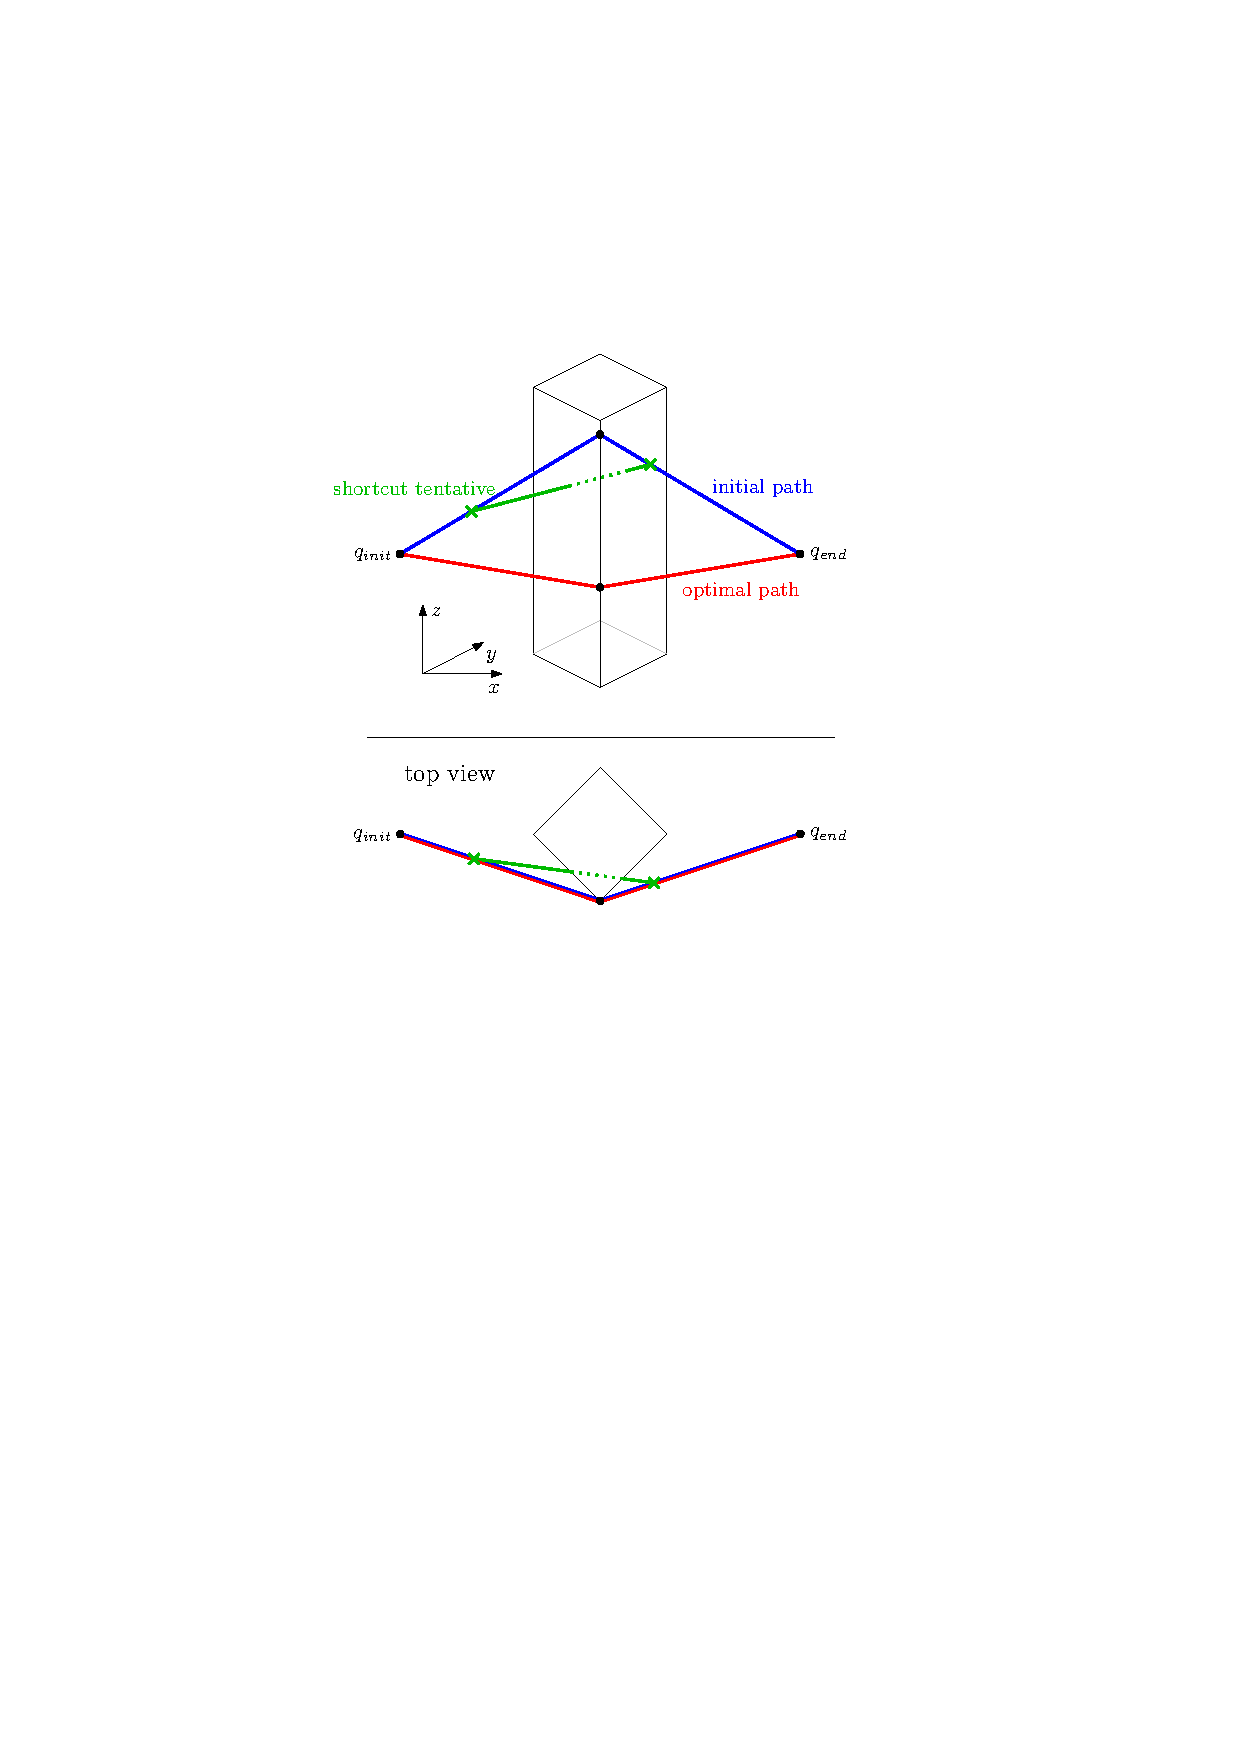
\includegraphics[width=7.5cm]{decoupled_DOF_optimization.pdf}
	\caption{Example of a path in $\real^3$ which random shortcut will never manage to 
	optimize: each shortcut attempt will provide a collision or will not 
	decrease the path length. The optimal path belongs to the $x-y$ plane 
	containing $\conf_{init}$ and $\conf_{final}$.}
	\label{decoupled_DOF_optimization}
\end{figure}



Finally it should be noticed that optimality in robot motion is a notion that should be clarified. Most of the 
time motion planners provide an optimized motion, which is not optimal at all, but is the output of a given 
optimization method. When optimal motions exist, numerical
algorithms mostly fail in accounting for their combinatorial structure. In addition, optimization algorithms 
bypass (not overcome) the question of the existence of optimal motions~\cite{LaumondOptim}. In that perspective, 
a path optimization algorithm has to be evaluated with respect to other existing optimization techniques, 
from qualitative properties and from computational performance.

The idea of our method is to find a good trade-off between
the simplicity of “blind” methods like shortcut algorithms,
and the complexity of distance based optimization techniques.
The method iteratively shortens the initial path with gradient-based information.
When a collision is detected at a given iteration, the method backtracks to the
latest valid iteration and inserts a one-dimensional constraint
between the objects detected in collision. Only collisions between objects are 
evaluated, therefore no pre-processing of either the
robot or environment models is necessary to increase distance computation speed. 
Respecting the problem geometry also 
preserves that a solution can still be found, e.g. for narrow passages as holes or 
grippers. The method is also repeatable since no randomness is introduced. The underlying optimization algorithm is a \textcolor{blue}{Linearly Constrained Quadratic Program (LCQP)}.

\textcolor{blue}{Another important feature of our contribution is that we optimize paths on the robot configuration space in a proper mathematical way. Most other optimization algorithms represent $SO(3)$ rotations by a vector directed along the rotation axis and the norm of which is the rotation angle, also known as the exponential map of $SO(3)$, or even worse by Euler angles.}

Related work is presented in Section II. Section III explains how the 
path-optimizer works, from the formulation of the problem to the implemented
algorithm. Finally, we conclude on experimental results in Section IV.

\section{RELATED WORK}
Previous work on path optimization has been conducted. CHOMP algorithm~\cite{chompIjrr} optimizes an initial guess provided as
input. It minimizes a time invariant cost function using efficient covariant
Hamiltonian gradient descent. The cost is quantified by non-smooth parts (with
high velocities) and an obstacle avoidance term, provided by the distance to the 
nearest obstacle for each iteration of the trajectory. Calculating these nearest 
distances however is time-consuming because the distances between all pairs of 
objects must be computed at each time step along the path. To reduce the 
computation time, the method starts by building offline a map of distances that 
will be called during the optimization at the requested time. Besides, meshes 
are pre-processed into bounding spheres so that distances are computed faster 
at the cost of a geometry approximation.

STOMP method~\cite{KalakrishnanStomp} avoids to compute an 
explicit gradient for cost optimization using a stochastic analysis of local 
random samples. But as for CHOMP, the obstacle cost term requires a voxel map to 
perform its Euclidean Distance Transforms, and represents the robot bodies with 
overlapping spheres. Such technique provides lots of distance and penetration 
information but remains very time consuming and is not as precise as some 
distance computation techniques based on the problem meshes as 
Gilbert-Johnson-Keerthi~\cite{gilbertGjk}.

Some optimization-based planners may not require an initial guess but some naive 
straight-line manually or randomly-sampled initialization as 
TrajOp~\cite{SchulmanConvexOptim}. The path is iteratively optimized with 
sequential convex optimization by minimizing at each step its square length, 
linear and non-linear constraints considered as penalties. To compute the 
collision-constraints, nearest obstacle distances are calculated at each discrete 
time of the trajectory vector. This can be a burden for a high-dimensional robot 
or a complex environment as we propose to use, and may be compensated with a 
short path composed of only one or two waypoints.


The elastic strips framework~\cite{BrockElasticStrips} is also an optimization 
based method. The path is modeled as a spring and obstacles give rise to a 
repulsive potential field. Although designed for on-line control purposes, this 
method may be used for path shortening. In this case however, the number of 
distance computation is very high. The authors also proposed to approximate the 
robot geometry by spheres.

Some heuristics use random shortcuts on the initial guess combined with a 
trajectory re-building. For example,~\cite{HauserFastSmooth} returns smooth shortcuts made of parabola and line combinations, relying on the classical bang-bang control approach. These local refined trajectories 
are time-optimal since they comply with acceleration and velocity constraints. 
Also based on random shooting,~\cite{Guernane2011} is guiding 
configuration-generation with local holonomic considerations. 
Nevertheless this method remains only 
locally optimal, and is not addressing high-DOF 
problems.~\cite{GeraertsIJRR07} is 
using medial axis retraction for clearance and a PRS (shortcut is applied only 
on some random DOF) 
which can address the problem of Figure~\ref{decoupled_DOF_optimization}. 
However it is 
relatively slower than RS, and~\cite{GeraertsIJRR07} only investigates 
it for freeflyer robots. 
Furthermore PRS is not taking advantage of information returned by 
the checker of which links are colliding, in order to guide the selection of a relevant group of DOF to shortcut.

In some way, our method shares similarities with~\cite{PanSmoothSplineShort} 
since this latter work relies on collision checking and backtracks when an 
iteration is detected in collision, instead of trying to constantly satisfy 
distance constraints. Unlike our method however, collision constraints are 
handled by interpolating configurations which, at some points of the trajectory, 
freeze the whole robot configuration instead of a pertinent subpart. Thus, this 
method cannot solve Figure~\ref{decoupled_DOF_optimization} issue.


\section{PATH OPTIMIZATION} \label{section:path_optim}

\textcolor{blue}{This section describes the establishment of the Gradient-based optimizer. The method works as a classical Linearly Constrained Quadratic Program (LCQP), reducing the path length expressed as a cost function and avoid collisions with linearized constraints. Details of the LCQP elements will be given in the following subsections, and associated to functions that will populate the algorithm, presented in the last section.}

\subsection {Kinematic chain}

A robot is defined by a kinematic chain composed of a tree of joints. We denote 
by $(J_1,\cdots,J_m)$ the ordered list of joints. Each joint $J_i$, $i=1\cdots m$, is represented by a mapping from a sub-manifold of $\real^{n_i}$, where $n_i$ 
is the dimension of $J_i$ in the configuration space, to the space 
of rigid-body motions $SE(3)$. The rigid-body motion is the position of the joint 
in the frame of its parent. In the examples presented in this paper, we consider four 
types of joints described in (Table~\ref{tab:joints}).
\begin{table}
\centerline {
  \begin{tabular}{cccc}
    Name & dimension & config space & velocity\\
    \hline
    translation & 1 & $\real$ & $\real$\\
    bounded rotation & 1& $\real$ & $\real$\\
    unbounded rotation & 2 & $\Sone\subset\real^2$ & $\real$\\
    $SO(3)$ & 4 & $\Sthree\subset\real^4$ & $\real^3$
  \end{tabular}
}
\caption {Translation and rotation joints positions are defined by one 
parameter corresponding respectively to the translation along an axis and a 
rotation angle around an axis. Unbounded rotation is defined by a point on the 
unit circle of the plane: two parameters corresponding to the cosine and the 
sine of the rotation angle. $SO(3)$ is defined by a unit quaternion. The 
velocity of translation and bounded rotation joints is the derivative of the 
configuration variable. The velocity of an unbounded rotation joint corresponds 
to the angular velocity. The velocity of a $SO(3)$ joint is defined by the 
angular velocity vector $\omega\in\real^3$.}
\label{tab:joints}
\end{table}
A configuration of the robot
$$\conf = (\underbrace{q_1,\cdots,q_{n_1}}_{J_1},\underbrace{q_{n_1+1},
\cdots,q_{n_1+n_2}}_{J_2},\cdots q_n),\ n\triangleq\sum_{i=1}^m n_i$$
is defined by the concatenation of the joint configurations. The configuration 
space of the robot is denoted by $\CS\subset\real^n$. Note that the configuration of the robot belongs to a sub-manifold of $\real^n$.

The velocity of each joint $J_i$, $1\leq i \leq m$,  belongs to the tangent space of 
the joint configuration space, and is defined by a vector of $\real^{p_i}$, where 
$p_i$ is the number of DOF of $J_i$. Note that
the velocity vector does not necessarily have the same dimension as the 
configuration vector.

The velocity of the robot is defined as the concatenation of the velocities of 
each joint:
$$\dot{\conf} = (\underbrace{\dot{q}_{1},\cdots,\dot{q}_{p_1}}_{J_1},
\underbrace{\dot{q}_{p_1+1},\cdots,\dot{q}_{p_1+p_2}}_{J_2},\cdots \dot{q}_p),\ p
\triangleq\sum_{i=1}^m p_i$$

\subsubsection{Operations on configurations and vectors}%
By analogy with the case 
where the configuration space is a vector space, we define the following 
operators between configurations and vectors:
$$
\conf_2 - \conf_1 \in \real^p, \ \conf_1, \conf_2\in\CS
$$
is the constant velocity moving from $\conf_1$ to $\conf_2$ in unit time, and
$$
\conf + \dot{\conf}\in\CS, \ \conf\in\CS \ \dot{\conf}\in\real^p
$$
is the configuration reached from $\conf$ after following constant velocity $
\dot{\conf}$ during unit time.

Note that the definitions above stem from the Riemanian structure of the 
configuration space of the robot. The above sum corresponds to the exponential 
map. The reader can easily state that ``following a 
constant velocity'' makes sense for the four types of joints defined in 
(Table~\ref{tab:joints}). We refer to~\cite{riemanian-optim2008} Chapter~5 for 
details about Riemanian geometry.

\subsection {Straight interpolation}

Let $\conf_1, \conf_2\in\CS$ be two configurations. We define the straight 
interpolation between $\conf_1$ and $\conf_2$ as the curve in $\CS$ defined on 
interval $[0,1]$ by:
$$
t \rightarrow \conf_1 + t (\conf_2 - \conf_1)
$$
This interpolation corresponds to the linear interpolation for translation and 
bounded rotations, to the shortest arc on $\Sone$ for unbounded rotation and to 
the so called slerp interpolation for $SO(3)$.

\subsection{Problem definition}

We consider as input a path composed of a concatenation of straight 
interpolations between $wp+2$ configurations: $(\conf_0, \conf_1,\cdots,\conf_{wp
+1})$. This path is the output of a random sampling path planning algorithm 
between $\conf_0$ and $\conf_{wp+1}$. We wish to find a sequence of waypoints $
\conf_{1}$,...,$\conf_{wp}$ such that the new path $(\conf_0, \conf_1,\cdots,
\conf_{wp+1})$ is shorter and collision-free. Note that $\conf_0$ and $\conf_{wp
+1}$ are unchanged and that the workspace of the robot contains obstacles. We 
denote by $\xx$ the optimization variable:
$$
\xx \triangleq (\conf_1,\cdots,\conf_{wp})
$$

Each path $\xx$ is a mapping from 
interval $[0,1]$ into $\CS$: $\xx(0) = q_0$, $\xx(1) = q_{wp+1}$.
Finally, we use a continuous 
collision checker inspired of~\cite{SchwarzerExactCollision} to validate our 
paths and to return the first colliding configuration 
\textcolor{blue}{and its abcissa} along a path.

\subsubsection{Cost}
Let $W\in\real^{p\times p}$ be a diagonal matrix of weights:
$$
W=\left(\begin{array}{cccccccccc}
w_1 I_{p_1}       &        &  0  \\
    & w_2 I_{p_2} &        &   \\
    &            & \ddots &   \\
  0 &            &        & w_m I_{p_m}
\end{array}\right)
$$
where $I_{p_i}$ is the identity matrix of size $p_i$ and $w_i$ is the weight 
associated to the joint $J_i$. We define the length of the straight interpolation 
between two configurations as:
$$
\|\conf_2 - \conf_1\|_{W} \triangleq \sqrt{(\conf_2 - \conf_1)^T W^2 (\conf_2 - 
\conf_1)}
$$
Weights are used to homogenize translations and rotations in the velocity vector. 
For a rotation, the weight is equal to the maximal distance of the robot bodies 
moved by the joint to the center of the joint, in a given configuration.

Given $\conf_0$ and $\conf_{wp+1}$ fixed, the cost we want to minimize is defined 
by
$$
\cost (\xx) \triangleq \frac{1}{2}\sum_{k=1}^{wp+1} \lambda_{k-1} \|\conf_{k}-\conf_{k-1}\|_{W}
^{2}
$$
where the $\lambda_{k-1}$ coefficients will be explained in the results 
section. For now it is assumed that $(\lambda_{k-1})_{k=1\cdots wp+1}=1$. Note that 
$\cost$ is not exactly the length of the path, but it can be 
established that minimal length paths also minimize $\cost$. This latter cost is 
better conditioned for optimization purposes.

The gradient of the cost function $\nabla \cost (\xx)$ is computed as follows:
$$
\nabla \cost (\xx) = 
\left( (\lambda_{k}(\conf_{k+1} - \conf_{k})^T - \lambda_{k+1}(\conf_{k+2} - \conf_{k+1})^T) \weight^2 \right)_{k=0\cdots wp-1}
$$


From the gradient expression, we notice that the Hessian $\mbox{H}$ is constant:
$$
\mbox{H} = \left(\begin{array}{cccccc}
(\lambda_{0}+\lambda_{1})\weight^2 & -\lambda_{1}\weight^2 & 0 & \cdots & & 0 \\
-\lambda_{1}\weight^2 & (\lambda_{1}+\lambda_{2})\weight^2 & -\lambda_{2}\weight^2 & 0 & \cdots & 0 \\
0 & -\lambda_{2}\weight^2 &  (\lambda_{2}+\lambda_{3})\weight^2 & -\lambda_{3}\weight^2 & 0 & \vdots \\
\vdots & \ddots & \ddots & \ddots & \ddots & \vdots\\
\vdots & & \ddots & \ddots & \ddots & \vdots\\
0 & \cdots  & 0 & -\lambda_{wp-2}\weight^2 & (\lambda_{wp-2}+\lambda_{wp-1})\weight^2 & -\lambda_{wp-1}\weight^2 \\
0 & \cdots &  \cdots & 0 & -\lambda_{wp-1}\weight^2 & (\lambda_{wp-1}+\lambda_{wp})\weight^2  \\
\end{array}\right)
$$

\subsection {Resolution}
We assume that the direct interpolation between the initial and final configurations contains collisions. An iteration at stage $i$ is described as follow:
\begin{equation}\label{eq:iteration-1}
\begin{split}
& \p_i =  -\mbox{H}^{-1} \nabla \cost(\xx_i)^{T} \\
& \xx_{i+1} =  \xx_{i} + \alpha_i \p_i
\end{split} 
\end{equation}
where \textcolor{blue}{$\p_i$ is computed by an unconstrained version of function \texttt{computeIterate}, and} $\alpha_i$ is a real-valued parameter. Taking $\alpha_i=1$ yields the 
unconstrained minimal cost path, i.e. all waypoints aligned on the straight line 
between $\conf_0$ and $\conf_{wp+1}$. Since this solution is in collision, we set 
$\alpha_i = \alpha_{init}$
where $\alpha_{init}$ is a parameter in interval $[0,1]$.

We iterate step~(\ref{eq:iteration-1}) until path $\xx_{i+1}$ is in collision.
When a collision is detected, we introduce a constraint and perform a new 
iteration from $\xx_i$ as explained in the next section.

\subsection{Linear Constraints}

\begin{figure}
	\centering
	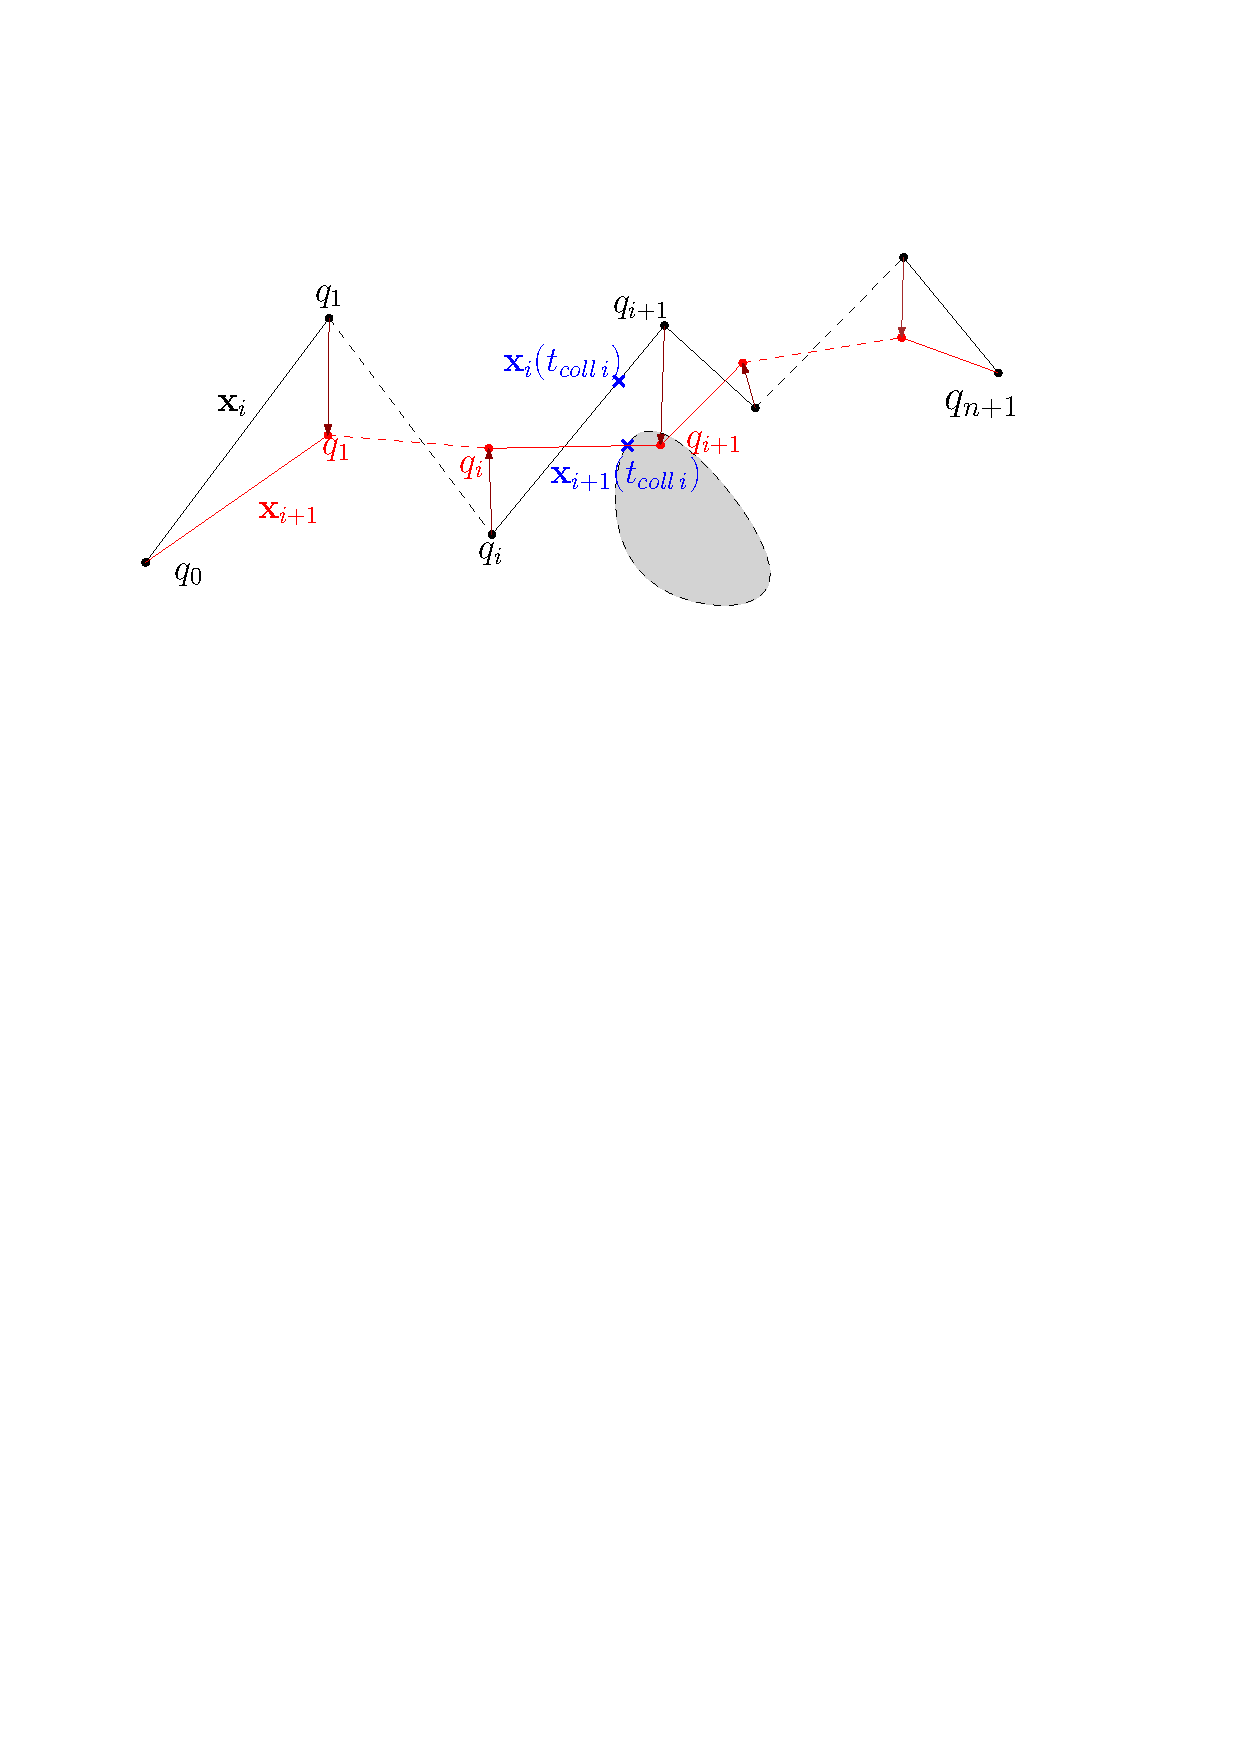
\includegraphics[width=9cm]{optim_grad.pdf}
	\caption{Illustration of one iteration of our optimization.
	$\xx_{i+1}$ appears 
	to be in collision with the obstacle. The first colliding configuration 
	$\xx_{i+1}(\tcolli)$ \textcolor{blue}{at abcissa $\tcolli$} is returned by 
	the continuous collision checker. The 
	corresponding constraint will be computed in the backtracked configuration 
	$\xx_{i}(\tcolli)$.}
	\label{optim_grad}
\end{figure}

Let us assume that at iteration $i$, $j$ \textcolor{blue}{linear} constraints have been inserted before the current iteration. 
These constraints are stored as lines of a matrix as follows:
$$
\Jf_{i} = \left(\begin{array}{c}L_1 \\ \vdots \\ L_j\end{array}\right)
$$
where the step $\p_i$ is constrained to be in the kernel of $\Jf_{i}$ as follows:
$$
\Jf_{i} \, \p_i = 0
$$
\textcolor{blue}{These linear constraints are built from the linearization of a collision-constraint function, which will be detailed in the following section.}

\subsubsection{New constraint}\label{subsubsec:new-constraint}

As illustrated in Figure~\ref{optim_grad}, let 
us denote by $\tcolli$ the abscissa of the first collision detected on path 
$\xx_{i+1}$, which previous iteration $\xx_i$ was collision-free. Thus in 
configuration $\xx_{i+1}(\tcolli)$ a collision has been 
detected. Two cases are possible:
\begin{enumerate}
\item the collision occurred between two bodies of the robot: $\body_1$ and $
\body_2$, or
\item the collision occurred between a body of the robot $\body_1$ and the 
environment.
\end{enumerate}
In the rest of this section, the first case only will be considered. Reasoning 
about the second case is similar, except that the 
constraint is on the position of $\body_1$ with respect to the environment.

\begin{figure}
	\centering
	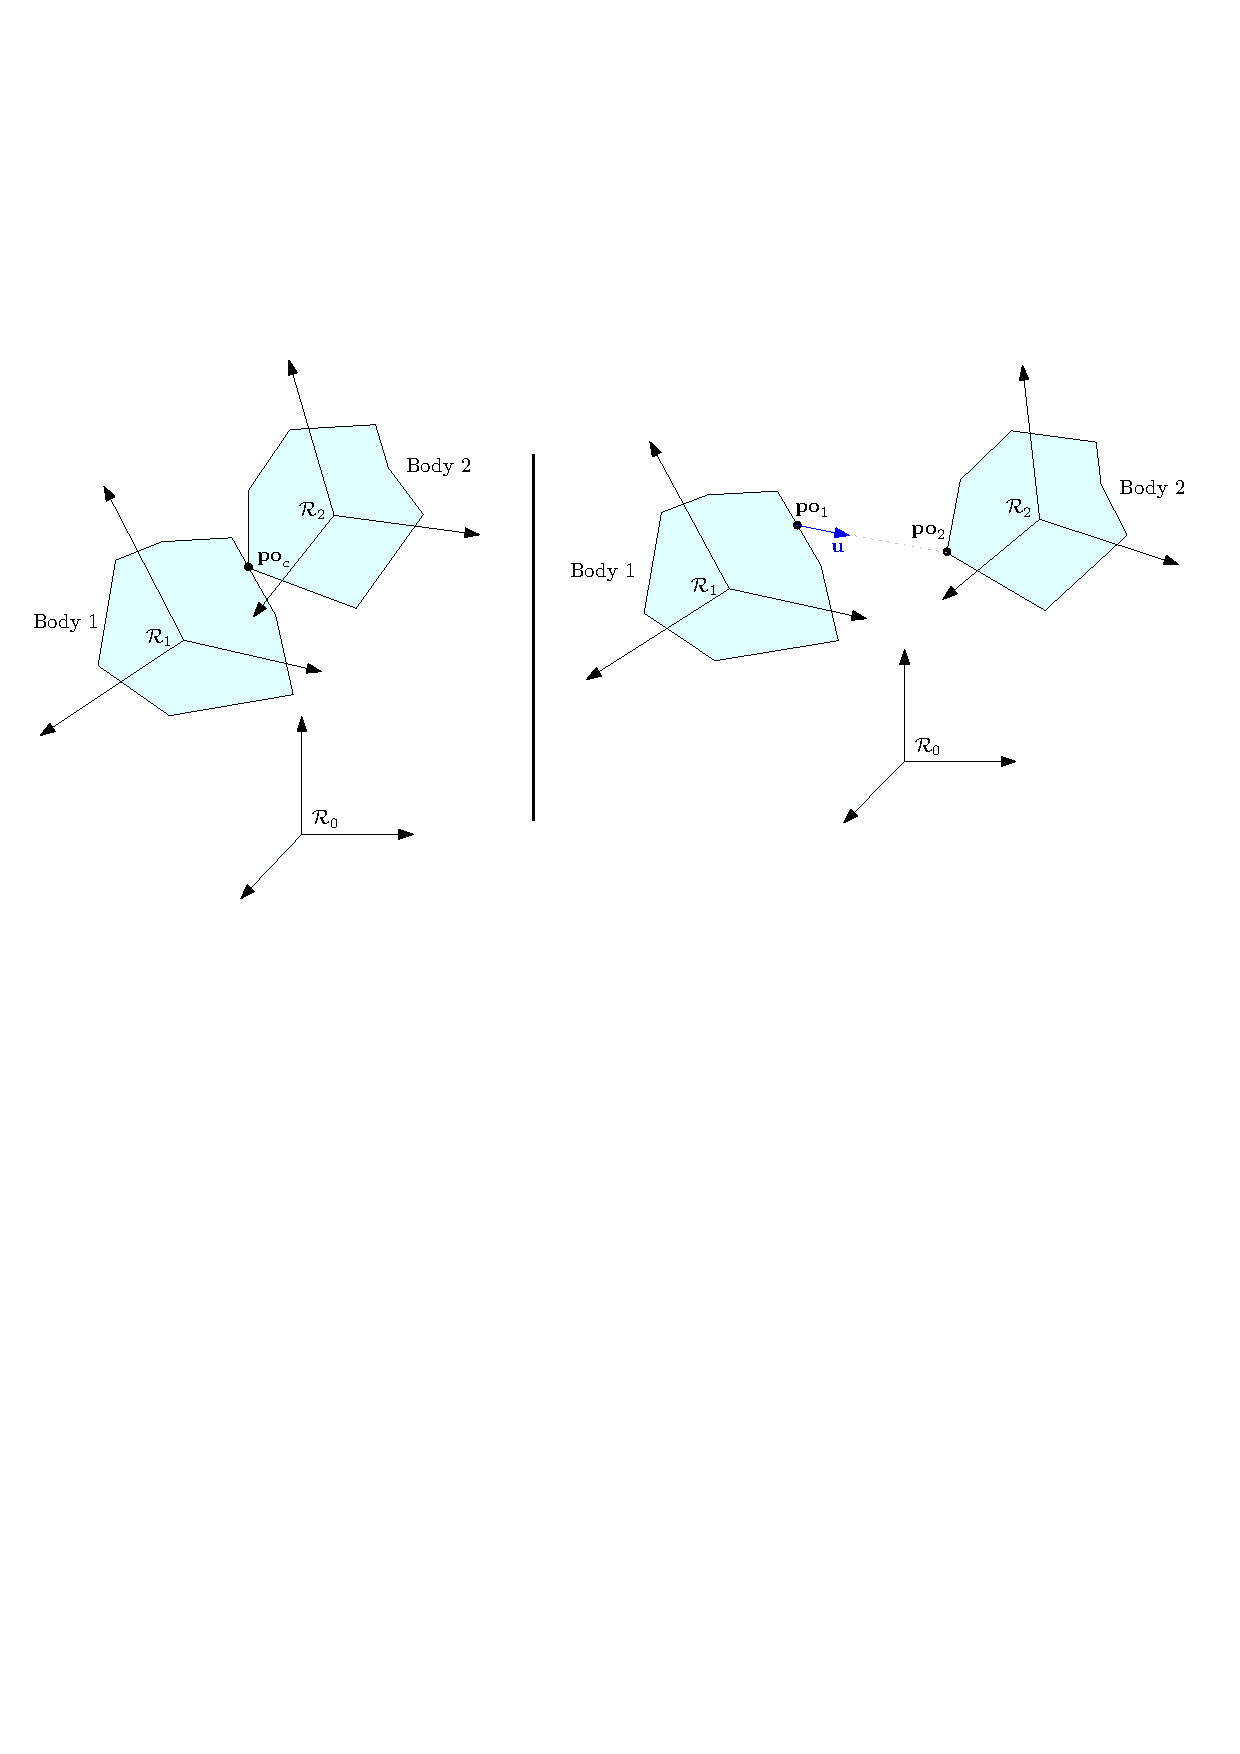
\includegraphics[width=15.8cm]{contact-points.pdf}
	\caption{Bodies representation in collision-configuration (left) and 
	backtracked collision-free configuration (right). A contact point (i.e. any point in 
	the intersection of the bodies) $\po_c$ can be returned by the Flexible 
	Collision Library~\cite{fcl}, used to detect collisions. 
	\textcolor{blue}{Constraint defined by~\eqref{eq:new-constraint} aims at 
	keeping $\po_2(\conf)$ in plane $\Pi$ fixed to $\body_1$.}
	}
	\label{contact-points}
\end{figure}

The principle of the method is to compute a \textcolor{blue}{linear} constraint, 
initialized on the 
collision-free configuration $\xx_{i}(\tcolli)$ to avoid the encountered collision $\xx_{i+1}
(\tcolli)$. To handle this, we introduce a one-dimensional constraint based on the 
orthogonal direction of the encountered collision.

In the collision-configuration $\xx_{i+1}(\tcolli)$, let $\po_c\in \real^3$ be a 
contact point expressed in the global frame 
(Figure~\ref{contact-points} left).
\textcolor{blue}{We denote by:
  \begin{itemize}
  \item $\po_1^{loc}$ (resp. $\po_2^{loc}$) the coordinate vector of $\po_c$ in the local frame of  $\body_1$ (resp. $\body_2$),
  \item $M_1(\conf) \in SE(3)$ (resp. $M_2(\conf) \in SE(3)$) the rigid-body transformation representing the position of $\body_1$ (resp. $\body_2$) in the global frame, in configuration $\conf$,
  \item $M_2^1 (\conf) = M_1(\conf)^{-1} M_2(\conf)$ the position of $\body_2$ local frame in $\body_1$ local frame in configuration $\conf$,
  \item $\po_1(\conf)$ (resp. $\po_2(\conf)$) the points moving with $\body_1$ (resp. $\body_2$) of local coordinate $\po_1^{loc}$ (resp. $\po_2^{loc}$) in $\body_1$ (resp. $\body_2$) local frame.
  %% \item $\rotation_1(\conf) \in SO(3)$ (resp. $\rotation_2(\conf) \in SO(3)$) the rotation associated with $M_1(\conf)$ (resp. $M_2(\conf)$).
  \end{itemize}
We define $\U$ as the coordinate vector of the unit vector linking points $\po_1$ and $\po_2$ in configuration $\xx_{i}(\tcolli)$, expressed in local frame of $\body_1$ (Figure~\ref{contact-points} right):
$$
\U = \frac{M_2^1 (\xx_{i}(\tcolli))\po_2^{loc} - \po_1^{loc}}{\|M_2^1 (\xx_{i}(\tcolli))\po_2^{loc} - \po_1^{loc}\|}
$$
Note that $\U$ is well defined since configuration $\xx_{i}(\tcolli)$ is collision-free.
}
\textcolor{blue}{
  Let $g$ be the real valued function mapping the projection of vector $\overrightarrow{\po_1\,\po_2(\conf)}$ on $\mathbf{u}$ to a configuration $\conf$ . For any $\conf \in \CS$:
\begin{equation}\label{eq:g}
g (\conf) = \left(M_2^1 (\conf)\po_2^{loc} - \po_1^{loc} | \U\right)
\end{equation}
}
%which is calculated from the last collision-free path at abscissa $\tcolli$.

Let $f$ be the function defined from $\CS^{wp}$ to $\real$ by:
\begin{equation}\label{eq:f}
f (\xx) = g(\xx (\tcolli))
\end{equation}
\textcolor{blue} {The constraint defined for any path $\xx$ by:
\begin {equation}\label{eq:new-constraint}
f(\xx) - f(\xx_{i}) = 0.
\end {equation}
aims at keeping point $\po_2(\conf)$ in a plane fixed to $\body_1$, orthogonal to $\U$ and and passing by $\po_2$ in configuration $\xx_i(\tcolli)$ (Figure~\ref{contact-points} right).
}
We linearize the constraint around $\xx_{i}$: 
$$
\frac{\partial f}{\partial \xx}(\xx_i)(\xx - \xx_i) = 0
$$
The computation of the linearized constraint is described in the next
section. Then, a line is added in the constraint Jacobian matrix $\Jf_i$:
\begin {align*}
\Jf_{i+1} &= \left(\begin{array}{c}L_1 \\ \vdots \\ L_{j+1}\end{array}\right)\ \mbox {with}\\
L_{j+1} &= \frac{\partial f}{\partial \xx}(\xx_i)
\end{align*}
\textcolor{blue}{This stage is performed by a function \texttt{addCollisionConstraint}}.

\vspace{0.4cm}

Finally, we refer to~\cite{nocedal2006numerical} for solving \textcolor{blue}{LCQP. The step computation corresponds to a constrained 
version of \texttt{computeIterate}}.

%The solution step is given by:
%$$
%\mathbf{\pii}^{*} = -V_0(V_0^TH V_0)^{-1}\,V_0^T\nabla c(\xx_i)
%$$
%where $V_0$ is the base of the nullspace of the stack of $J_F$ jacobians.

\vspace{0.2cm}

\subsubsection{Linearized constraint computation} \label{sec:lin_constr_compt}

Let $\conf_{k,i}$ denote the waypoint $k$ along path $\xx_i$.
There exist $\beta\in[0,1]$ and $k$ such that $\xx_i (\tcolli)$ can be written as a combination of two waypoints:
$$
\xx_i (\tcolli) = \conf_{k,i} + \beta (\conf_{k+1,i} - \conf_{k,i})
$$

Thus the linearized constraint Jacobian $\frac{\partial f}{\partial \xx}(\xx_i)$ 
is built by matrix 
blocks using the Jacobian $\frac{\partial f}{\partial \conf}$ expressed in 
each of the two waypoints and $\beta$. \textcolor{blue}{This stage is performed by \texttt{computeCollisionConstraint}}.


\subsection{Convergence Analysis and algorithm refinment}

\begin {figure}
  \centerline {
    \def\svgwidth {.7\linewidth}
    \graphicspath{{./images/}}
    \input {images/convergence.pdf_tex}
  }
  \caption {\textcolor{blue}{Illustration of linearly constrained quadratic program on a problem analogous to the path shortening problem: we want to minimize the quadratic cost $\frac{1}{2}\|\xx-\xx^*\|^2, \xx\in\real^2$ under the non-linear constraint $f(\xx)\leq 0$. $\alpha_{init}=\frac{1}{4}$. The algorithm starts from $\xx_0$. The first iterate is $\xx_1$ which satisfies the constraint. The second iterate is $\xx_2$ that does not satisfy the constraint. The algorithm backtracks to $\xx_1$ and inserts linear constraint $L_1: \frac{\partial f}{\partial \xx} (\xx_1)(\xx - \xx_1) = 0$. $\xx_3$ is the global minimum under $L_1$. As $\xx_3$ does not satisfy the constraint, the algorithm moves to $\xx_4$ that satisfies the constraints, and then to $\xx_5$ that does not. The algorithms backtracks to $\xx_4$, inserts constraint $L_2: \frac{\partial f}{\partial \xx} (\xx_2)(\xx - \xx_2) = 0$, and returns $\xx_4$ as a solution since the dimension of the search space is 0. Notice that the same non-linear constraint may give rise to several linear constraints. The convergence of the algorithm relies on the fact that the kernel of constraint $L2$ is not contained in the kernel of the current constraints ($L_1$ only here). The convergence analysis can be roughly summarized as follows. $L2$ to be linearly dependent of $L_1$ requires that $f$ is stationary along $L_1$ at $\xx_4$. This is unlikely (but possible) since $\xx_4$ is not far from the boundary of the domain defined by $f(\xx) \leq 0$. If $L_2$ was not linearly independent from $L_1$, The algorithm would keep searching new iterates between $\xx_5$ and $\xx_4$. If by any chance constraint $f$ linearized around each of those collision-free iterates was each time linearly dependent from $L_1$ the iterates would converge to the boundary of the domain defined by $f(\xx) \leq 0$. By continuous differentiability of $f$, this would mean that $f$ is stationary at the boundary. In other words, the straight line passing by $\xx_1$ and $\xx_3$ would cross the boundary tangently (as in bottom right picture). This is possible but unlikely, unless the problem has been defined as such on purpose.}}
  \label {fig:convergence}
\end{figure}

Although linearized constraints may differ from the initial geometrically relevant non-linear constraint when the iterate goes away from the linearization path, we will show in this section that  our algorithm converges under some reasonable assumptions. The underlying idea of the proof is sketched in Figure~\ref{fig:convergence}.

From the definition of $\Jf_{i}$, it is straightforward that:
\begin{equation}\label{eq:decreasing-kernel}
\kernel \Jf_{i+1} \subset \kernel \Jf_{i}
\end{equation}
Let us assume that:
\begin{equation}\label{eq:assumption-1}
L_{j+1}\p_i \not= 0
\end{equation}
We will elaborate later on this assumption. This means that 
$\p_{i}\notin\kernel \Jf_{i+1}$, and as $\p_{i}\in\kernel \Jf_{i}$, then:
$$
\kernel \Jf_i \not= \kernel \Jf_{i+1}
$$
From~(\ref{eq:decreasing-kernel}), we deduce that:
$$
\dim (\kernel \Jf_{i+1}) < \dim (\kernel \Jf_i)
$$
This result proves that under assumption~(\ref{eq:assumption-1}), each additional constraint is linearly independent from the 
previous ones, and thus our algorithm terminates in a finite number of iterations.

\subsubsection{Note about assumption~(\ref{eq:assumption-1})}%
\noindent
\textcolor{blue}{As in the previous section, we assume that $\xx_i$ is collision-free and that $\xx_{i+1}$ is in collision at abscissa $\tcolli$.
According to~(\ref{eq:f}), the evaluation of the constraint function $f$ along the iteration line $\xx_i + t\alpha_i \p_i,\ t\in [0,1]$ going from $\xx_i$ to $\xx_{i+1}$ can be written as follows:
\begin{equation}\label{eq:f-along-pi}
f (\xx_i + t\alpha_i \p_i) = g \left((\xx_i + t\alpha_i \p_i)(\tcolli)\right).
\end{equation}
The argument of function $g$ above is a trajectory in the robot configuration space that we denote by $\traj$:
\begin{equation}\label{eq:trajectory}
\traj (t) = (\xx_{i} + t\, \alpha_i \p_{i}) (\tcolli), \ t \in [0,1]
\end{equation}
The trajectory $\traj(t)$ is defined by taking the constant abscissa $\tcolli$ and by 
moving from 
path $\xx_i$ along step $\p_i$ (see Figure~\ref{fig:convergence-diagram}). Note that configuration $\xx_{i+1}(\tcolli)$ is reached when $t=1$.
Substituting~(\ref{eq:trajectory}) into~(\ref{eq:f-along-pi}) and differentiating with respect  to $t$ yields
\begin{align}
f (\xx_i + t\alpha_i \p_i) &= g (\traj (t)) \\
\label{eq:df/dx}
\alpha_i \frac{\partial f}{\partial \xx} (\xx_i + t\alpha_i \p_i)\p_i &=
\frac{d}{dt}g (\traj (t))
\end{align}
\begin{property}\label{prop:geometric-reasoning}
From the definition~(\ref{eq:g}) of $g$, the right hand side of~(\ref{eq:df/dx}) represents the velocity of point $\po_2$ in reference frame $\body_1$ projected on vector $\U$.
\end{property}
}

\begin{figure}
	\centering
	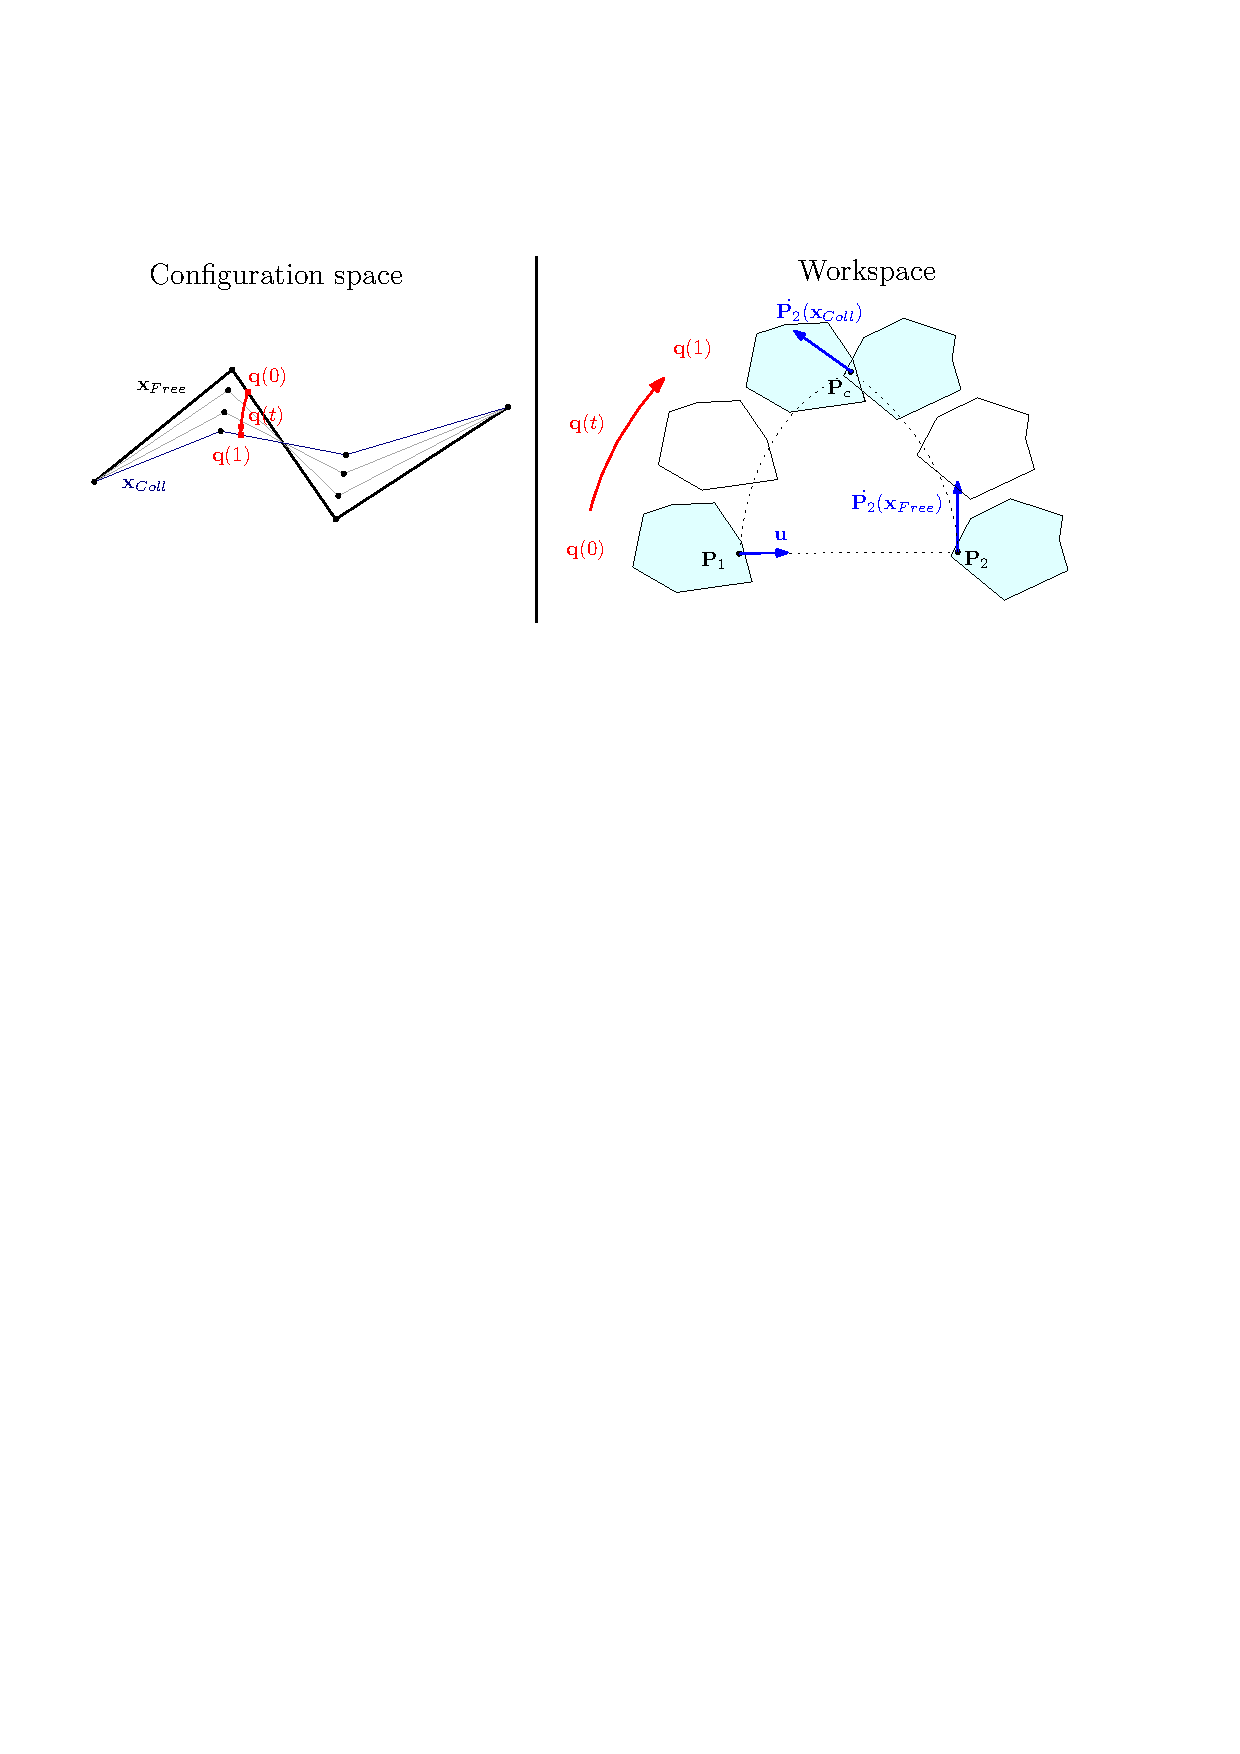
\includegraphics[width=8cm]{convergence-diagram2.pdf}
	\caption{\textcolor{blue}{Representation in the robot configuration space of the trajectory $\traj$, defined in Equation~\eqref{eq:trajectory}.}}
	\label{fig:convergence-diagram}
\end{figure}

\textcolor{blue}{
Therefore the following expressions
\begin{align*}
\alpha_i \frac{\partial f}{\partial \xx} (\xx_i)\p_i = \frac{d}{dt}g (\traj (0)) & &
\alpha_i \frac{\partial f}{\partial \xx} (\xx_{i+1})\p_i =\frac{d}{dt}g (\traj (1))
\end{align*}
correspond to $(\velocity_{\po_2/\body_1}|\mathbf{u})$, respectively in configurations $\xx_{i}(\tcolli)$ and $\xx_{i+1}(\tcolli)$, where $\velocity_{\po_2/\body_1}$ represents the velocity of point $\po_2$ in reference frame $\body_1$. 
Note that Assumption~(\ref{eq:assumption-1}) is equivalent to the first above equality to be different from 0. According to the geometric interpretation, Assumption~(\ref{eq:assumption-1}) is violated if and only if $\velocity_{\po_2/\body_1}$ is orthogonal to $\U$. Although very unlikely, this case might appear for some new constraint. In this case, inserting constraint $L_{j+1}$ is useless since
$$
\kernel \Jf_i = \kernel \Jf_{i+1}
$$
}

\subsubsection {Algorithm refinment}

\begin{algorithm}[b]
\begin{algorithmic}%[1] % line numerotation
\INPUT{$\xx_{Free}$ latest collision-free path, $\xx_{Coll}$ current path with collisions, $\p$ current iteration step}
\OUTPUT{linearized constraint $\frac{\partial f}{\partial \xx} (\xx_{Free})$}
\Require constraint $\frac{\partial f}{\partial \xx} (\xx_{Free})$ built from $\xx_{Coll}$ would produce a rank loss in constraint Jacobian $\Jf$
\State $solved \gets false$
\While{($\textbf{not}(solved)$)}
	%\State $\p = \texttt{computeIterate}()$
	\State $\alpha \gets 0.5\alpha$
	\State $\xx \gets \xx_{Free} + \alpha\,\p$
	\If{(\texttt{validatePath}($\xx$))}
		\State $\xx_{Free} \gets \xx$
	\Else
		\State $\xx_{Coll} \gets \xx$
	\EndIf
	\State $\frac{\partial f}{\partial \xx} (\xx_{Free}) \gets$\texttt{computeCollisionConstraint}($\xx_{Coll}$, $\xx_{Free}$)
	\State $solved \gets$ \texttt{isFullRank}($\Jf$ , $\frac{\partial f}{\partial \xx} (\xx_{Free})$)
\EndWhile
\end{algorithmic}
\caption{Description of \texttt{findNewConstraint}() which returns a linearly 
independent constraint w.r.t. previous constraints stacked in $\Jf$.} 
\label{algo:solveRedundant}
\end{algorithm}

\textcolor{blue}{
When the new constraint is not linearly independent from the set of previous constraints, the algorithm enters an additional loop, performed by Algorithm~\ref{algo:solveRedundant}, in order to find a new constraint that is linearly independent. The loop keeps looking for paths along line segment $[\xx_{i},\xx_{i+1}]$ by dichotomy. A pair containing the latest free path and the latest path in collision, denoted by $(\xx_{Free}, \xx_{Coll})$ is stored along the loop. New iterations are chosen in the middle of this pair. 
\begin{itemize}
\item If the new path is collision-free, it replaces $\xx_{Free}$ in the pair.
\item If the new path is in collision, it replaces $\xx_{Coll}$ in the pair.
\end{itemize}
In both cases, a new constraint is built following the method described in Section~\ref{subsubsec:new-constraint}. Two cases are then possible:
\begin{enumerate}
\item at some point in the loop the new constraint is linearly independent from the previous constraints. The new constraint is added to $\Jf_{i}$ to give rise to $\Jf_{i+1}$, and the loop is interrupted, or
%the new constraint makes the dimension of the kernel decrease
\item each new constraint is linearly dependent from the previous constraints and the loop never ends.
\end{enumerate}
In the second case, the iterations of the loop converge to a path that we denote by $\bar{\xx}$. $\xx_{Free}$ and $\xx_{Coll}$ also both converge to $\bar{\xx}$. $\bar{\xx}$ necessarily lies at the boundary between free paths and paths in collision. Let us denote by $\bar{\kappa}$ the abscissa along $\bar{\xx}$ where $\body_1$ and $\body_2$ come to contact, and let us denote by $\bar{\po}$ the contact point.
}

\textcolor{blue}{
At each iteration, the new linear constraint
$$
L_{j+1} = \frac{\partial f}{\partial\xx} (\xx_{Free})
$$
is tested. As iterations $\xx_{Free}$ and $\xx_{Coll}$ tend toward $\bar{\xx}$, it can be established by a geometric reasoning analogous to Property~\ref{prop:geometric-reasoning}, that
$L_{j+1} \p_i$ tends to the norm of the velocity of point $\bar{\po}$ belonging to $\body_2$ in the frame of $\body_1$. The following property summarizes the result of this section.
}

\textcolor{blue}{
\begin{property}\label{prop:convergence}
As long as along iteration $\p_i$, the trajectory $(\xx_i+t\alpha_i\p_i)(\bar{\kappa})$ does not enter in collision with contact point velocity equal to 0 in the frame of $\body_1$, Algorithm~\ref{algo:solveRedundant} converges in a finite number of steps.
\end{property}
The above property means that the gradient-based algorithm described in this paper converges in all cases, except for ill-defined problems.
}

\subsection{Algorithm}

\begin{algorithm}[b]
\begin{algorithmic}%[1] % line numerotation
\INPUT{path to optimize $\xx_0$}
\OUTPUT{optimized collision-free path $\xx_0$}
\State $\alpha \gets \alpha_{init}$
\State $minReached \gets false$
\While{($\textbf{not}(noCollision \textbf{ and } minReached)$)}
	\State $\p = \texttt{computeIterate}()$
	\State $minReached = (||\p||<10^{-3} \textbf{ or } \alpha=1)$
	\State $\xx_1 \gets \xx_0 + \alpha\,\p$
	\If{(\textbf{not}(\texttt{validatePath($\xx_1$)}))}
		\State $noCollision \gets false$
		\If{$(\alpha \neq 1)$}
			\State \texttt{computeCollisionConstraint}($\xx_1$, $\xx_0$)
			\State \texttt{findNewConstraint}()
			\State \texttt{addCollisionConstraint}()
			\State $\alpha \gets 1$
		\Else
			\State $\alpha \gets \alpha_{init}$
		\EndIf
	\Else
		\State $\xx_0 \gets \xx_1$
		\State $noCollision \gets true$
	\EndIf
\EndWhile
\end{algorithmic}
\caption{Gradient-based (GB) algorithm for path-optimization.} \label{algo:gradient}
\end{algorithm}

In this section, the GB path-optimizer Algorithm~\ref{algo:gradient} is described
according to the previous steps definitions.
\textcolor{blue}{Remind that, the LCQP optimal step $\p$ computed by \texttt{computeIterate} is known.
The idea of the algorithm is to process iterations that reduce the path length according to the LCQP cost. If collision-constraints have been added to the LCQP, further iterations will comply with them. The algorithm stops whether the LCQP minimum is reached and collision-free. The collision detection on a path is handled by \texttt{validatePath}, which returns $true$ if the given path is collision-free.
}

\textcolor{blue}{
One main difficulty is to handle 
the scalar parameter $\alpha$ determining how much of the computed step  will be traveled along. 
As presented in Algorithm~\ref{algo:gradient}, $\alpha$ takes two values, $\alpha_{init}<1$ to process smaller steps or $1$ to go directly to the optimum. This latter case is interesting since, if this optimal path is collision-free, the algorithm has converged and returns the path as the solution.
Choosing to travel small steps from a valid path decrease the chances of being in collision. Besides if one occurs, the collision-constraint is computed on the last valid path, which is not too much deformed compared to the path that has collisions. As a result, collision-constraints are only computed (\texttt{computeCollisionConstraint}) and added (\texttt{addCollisionConstraint}) when performing a reduced iteration (i.e. $\alpha = \alpha_{init}$).
}

Note that even if the constraints are linearized, the algorithm converges.


\section{RESULTS}

This part gathers optimization results performed on the planning software 
Humanoid Path Planner~\cite{hpp}. Initial paths are obtained with two 
kinds of probabilistic planners: Visibility-PRM~\cite{visibility-prm} and 
RRT-connect~\cite{rrt-connect}. Unless another value is provided, $\alpha_{init}$ 
is set to 0.2. \textcolor{blue}{A further section provides a discussion on the $\alpha_{init}$ value setting.}

\subsection{From 2D basic examples}

\begin{figure}[b]
	\centering
	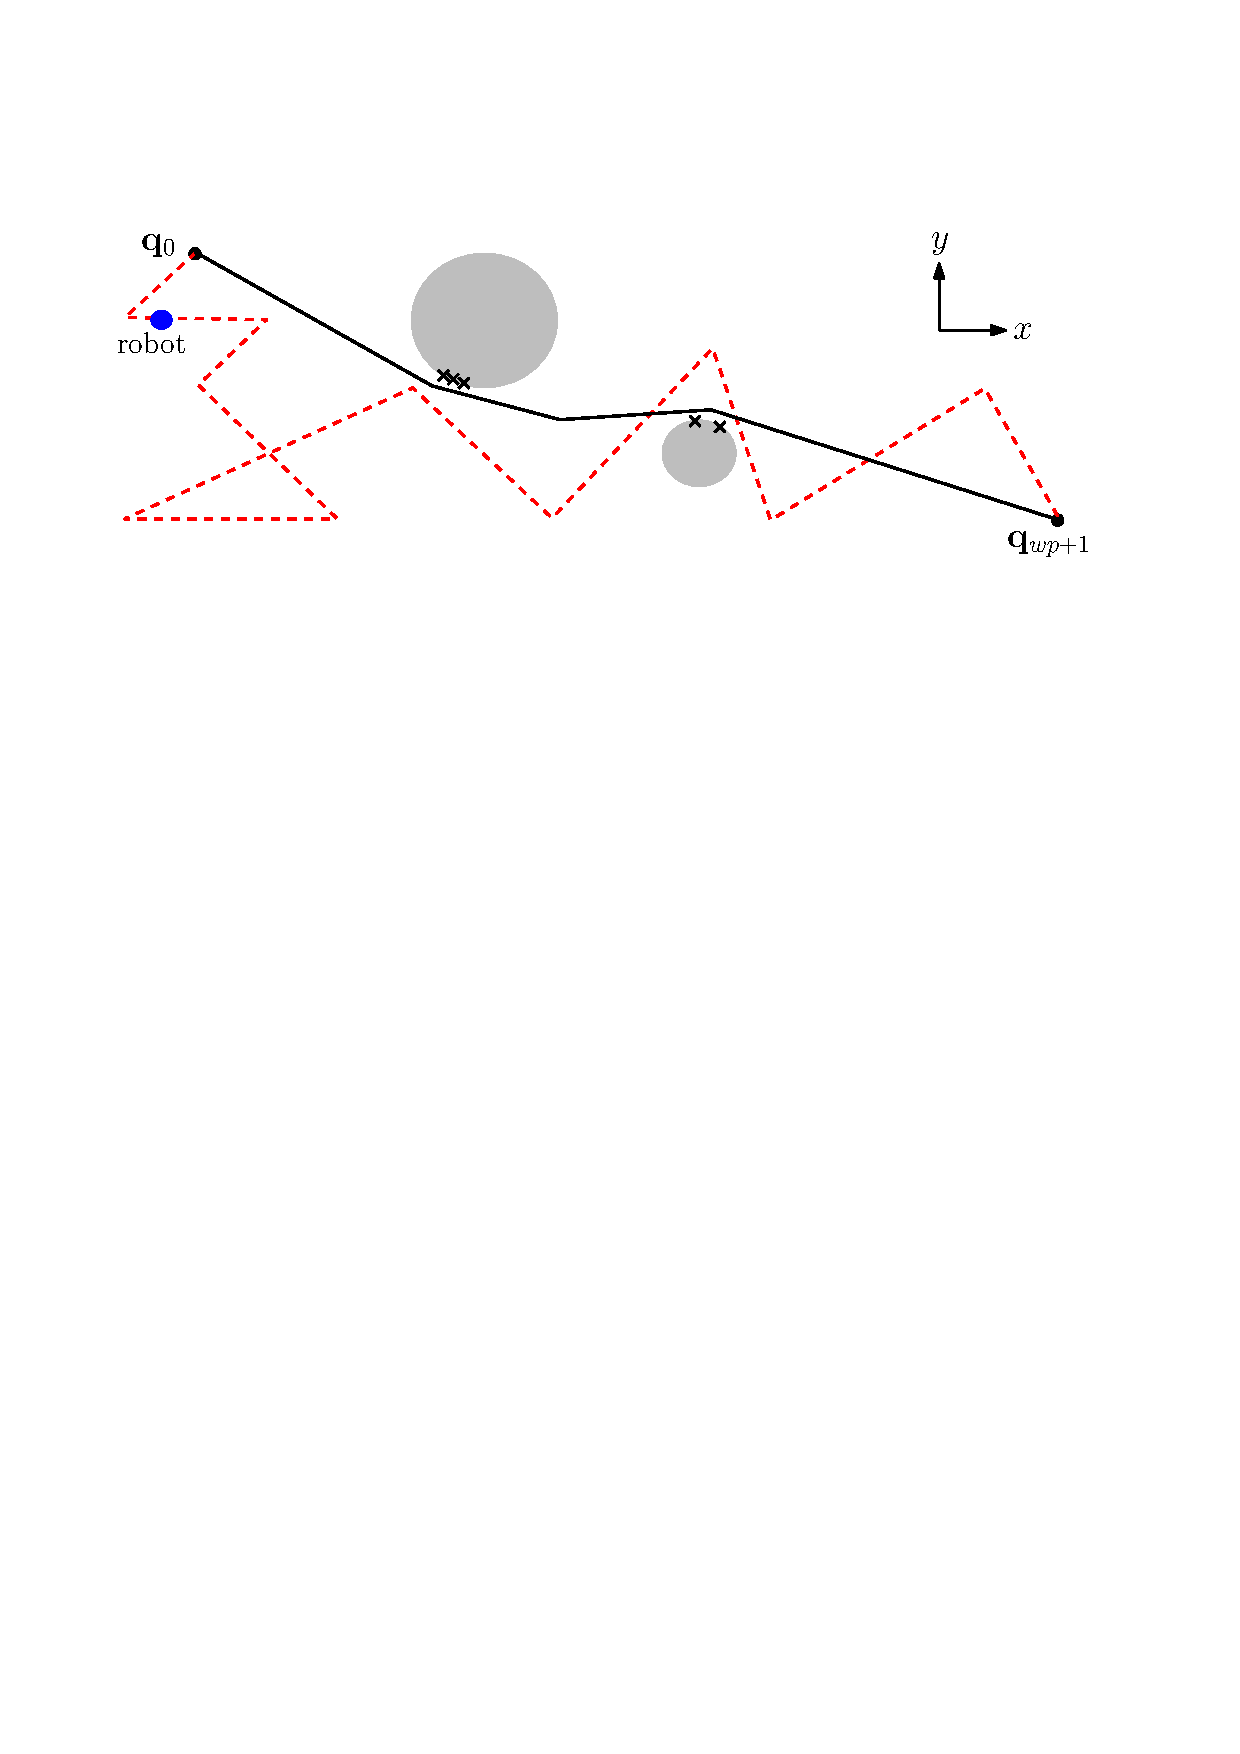
\includegraphics[width=7.8cm]{contact_points6.pdf}
	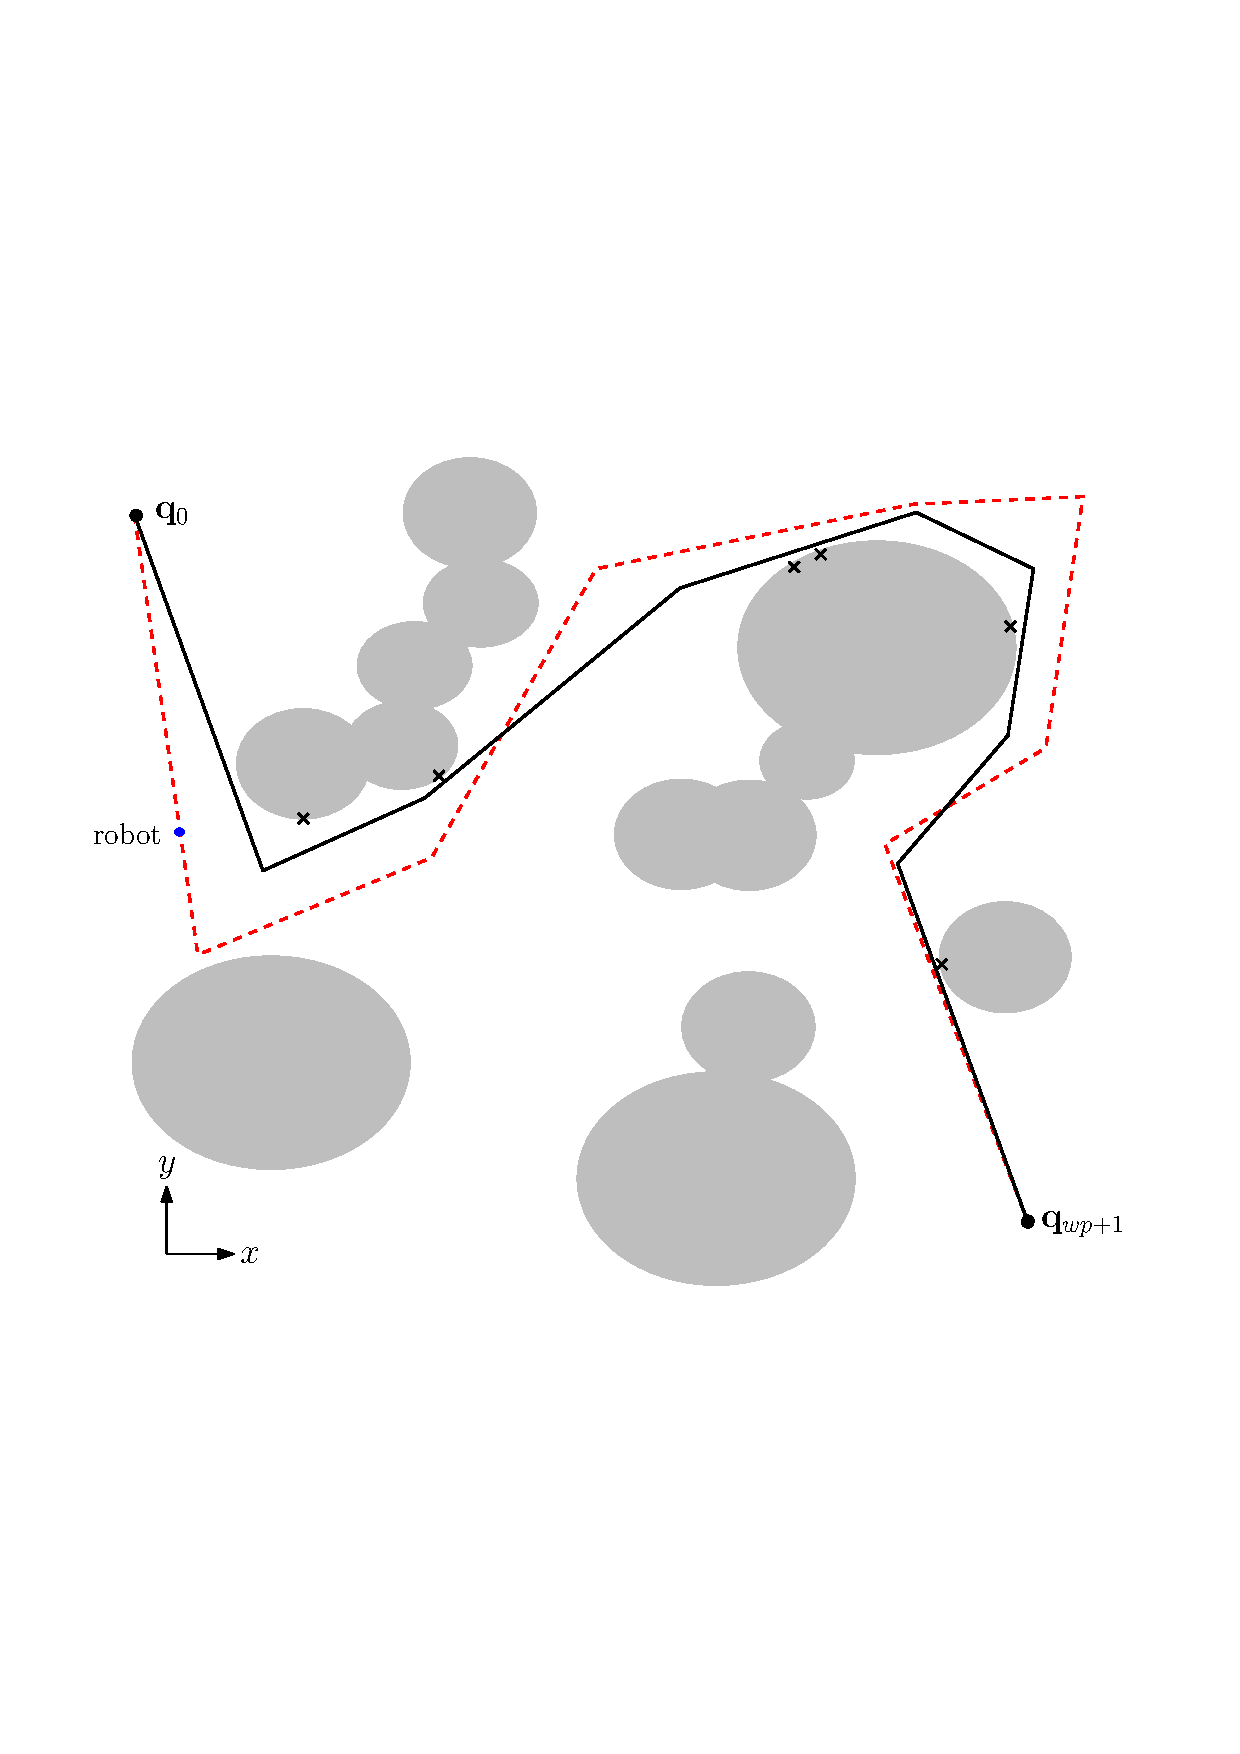
\includegraphics[width=8cm]{contact_points2potential.pdf}
	\caption{Path-optimization results on 2D robots, moving around 
	gray obstacles. Initial paths are dashed and crosses represent contact points 
	$\po_c$ related to collision-constraints. Note that, on the left, the detour 
	completely disappears.}
	\label{2D_long}
\end{figure}

Figure~\ref{2D_long} shows the result of our optimizer on 2D cases. Contact points which have 
led to constraints are represented. They permit to understand how the path is kept out of the obstacles. 
Unfortunately, it is not possible in the GB method to choose at which distance of the obstacle 
the constraint must be created, since at some parts the robot is very close to obstacles.

Besides, these examples give a better understanding of how the tuning of 
$\alpha_{init}$ 
has to balance lot of iterations and relevant collision-constraint addition. For 
example, if we alter a lot the initial path with a large gradient step and 
compute the corresponding collisions, constraints will be chosen on a 
path closer-to-optimality but which is not relevant
w.r.t. the obstacles we want to avoid.

Figure~\ref{local_box_optim} illustrates a \textit{very long} path example which RS 
or PRS will not manage to 
optimize in an affordable time, because of probabilistically failing to sample 
configurations in the box. The GB method succeeds to optimize the 
path contained in the box, with the following cost coefficients:
$$
\lambda_{k-1} = \frac{1}{\sqrt{(\conf_{k,0}-\conf_{k-1,0})^T \weight^2 
(\conf_{k,0}-\conf_{k-1,0})}}, \  k=1\cdots wp+1  
$$
aiming at keeping the same ratio between path segment lengths at 
minimum as at 
initial path, represented by the waypoints ($\conf_{i,0})_{k=1\cdots wp+1}$.
Without these coefficients, the path that minimizes the cost corresponds to a 
straight line with the waypoints equidistantly allocated. This is not relevant for 
Figure~\ref{local_box_optim} type of problems where a local passage is very
constrained by obstacles. Note that this cost is also working with all other 
examples presented in this paper, and provides better quality results than the original cost.



\subsection{To 3D complex problems}

\subsubsection{Comparison to random shortcut algorithms}
\begin{algorithm}
\begin{algorithmic}%[1] % line numerotation
\INPUT{Path to optimize $\xx$, time limit $t_{lim}$}
\OUTPUT{Optimized collision-free path $\xx$}
   \State \textcolor{blue}{$t_{start} \gets \texttt{currentTime()}; \ t \gets 0$}
   \While {\textcolor{blue}{$t < t_{lim}$}}
        \State $failure \gets true$
        \State $t_1 < t_2 \gets \mbox{random numbers in }[0,1]$
        \State $lp0 \gets \texttt{steeringMethod} (\xx(0), \xx(t_1))$
        \State $lp1 \gets \texttt{steeringMethod} (\xx(t_1), \xx(t_2))$
        \State $lp2 \gets \texttt{steeringMethod} (\xx(t_2), \xx(1))$
        \State $newPath \gets \mbox{empty path defined on }[0,0]$
   	\If{\texttt{validatePath($lp0$)}}
          \State $newPath \gets lp0$;
        \Else
          \State $newPath \gets \xx_{|[0,t_1]}$
        \EndIf
   	\If{\texttt{validatePath($lp1$)}}
          \State $newPath \gets \texttt{concatenate} (newPath, lp1)$
        \Else
          \State $newPath \gets \texttt{concatenate} (newPath, \xx_{|[t_1,t_2]})$
        \EndIf
   	\If{\texttt{validatePath($lp2$)}}
          \State $newPath \gets \texttt{concatenate} (newPath, lp2)$
        \Else
          \State $newPath \gets \texttt{concatenate} (newPath, \xx_{|[t_2,1]})$
        \EndIf
        \State $\xx \gets newPath$
        \State \textcolor{blue}{$t \gets \texttt{currentTime()} - t_{start}$}
      \EndWhile
    \Return $\xx$
\end{algorithmic}
\caption{Random shortcut as adapted from~\cite{Sekhavat-Svestka1998} 
Section~6.4.1. \texttt{steeringMethod} returns the linear interpolation between 
two configurations. $\xx_{|I}$ denotes path $\xx$ restricted to interval $I$. 
\textcolor{blue}{$t_{lim}$ represents the duration limitation of the algorithm.}}\label{algo:random-shortcut}
\end{algorithm}


Our algorithm is also experimented on more complex robots and environments.
In the included video and Figures~\ref{pr2_final},~\ref{fiad} 
and~\ref{fig:trajectories}, we present multiple situations where the GB algorithm 
is tested and compared to RS  and PRS.
\textcolor{blue}{
After describing the random optimizers, we will present each benchmark and its qualitative path results. Then quantitative averages and graphs will be given and discussed.
}

\textcolor{blue}{
The RS (see Algorithm~\ref{algo:random-shortcut}) shortens the path by randomly sampling configurations along it and trying to link them with collision-free interpolations.
The termination condition of RS is a duration time limit $t_{lim}$, and is typically set as the GB optimization duration.
%For our implementation of PRS, first a shortcut is tried on each DOF between $\conf_0$ and $\conf_{wp+1}$. % NOT ANYMORE
The implementation of PRS is identical to~\cite{GeraertsIJRR07}:
for a random DOF, configurations are sampled along the initial path as in 
Algorithm~\ref{algo:random-shortcut}. The steering-method returns a path 
made of an interpolation on only 
the current DOF and based on the previous subpath for other DOF. If this path is 
collision-free, it is added to the final path as in RS. The process is stopped when the duration exceeds $t_{lim}$.
}

\vspace{0.4cm}
% freeflyer puzzle
Before entering the manipulator examples, the GB algorithm is analyzed 
on a popular problem in the motion planning literature: a freeflyer puzzle, 
corresponding to Figure~\ref{fig:trajectories:puzzle}. The 
puzzle has to cross down the 
obstacle using the hole in the middle. The initial path planned with Visibility-PRM 
contains detours above and below the obstacle, as well as small superfluous
motions in the hole. 
The GB optimizer manages to modify the puzzle trajectory even in the hole, but remains less efficient than RS and PRS to shorten trajectories in the upper and lower parts. 
\textcolor{blue}{
This can be the result of adding collision-constraints on these parts of the trajectories, penalizing the global path length. One idea could be to 	arbitrarily cancel constraints in upper and lower parts, and keeping the ones in the hole. However we want the present GB algorithm to remain general and basic, such constraints relaxation are part of the future possible work.
}
%PRS fails to decrease the path length because in this problem, all DOF are closely related to cross the hole. This behavior was also noticed and improved in the PRS implementation of~\cite{GeraertsIJRR07}, acting on a group of DOF. The GB optimizer manages to modify the puzzle trajectory even in the hole, contrary to RS which simply copies the initial path when the trajectory gets near of the obstacle. 

\vspace{0.4cm}

% double-arm:
In the double-arm benchmark (4-DOF), 
Figure~\ref{fig:trajectories:double_arm}, one arm has 
to get around a cylinder obstacle while the 
other arm stay in the same configuration. As expected, the initial path given by 
RRT-connect activates both arms to solve the problem. Unlike RS, 
the GB optimizer manages to cancel the rotation of the free-arm while optimizing 
the first arm motion, creating collision-constraints with the cylinder obstacle.


\begin{figure}
	\centering
	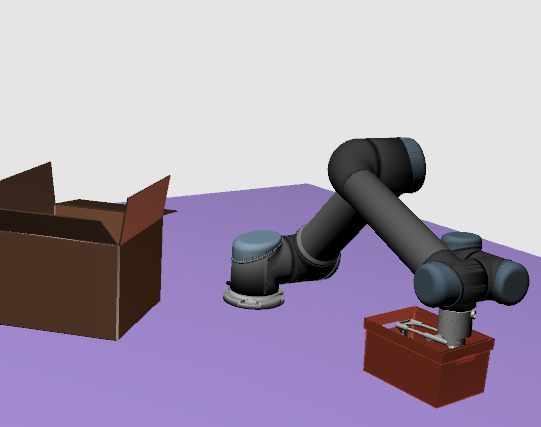
\includegraphics[width=5.8cm,height=4.7cm]{fiad_qinit.png}
	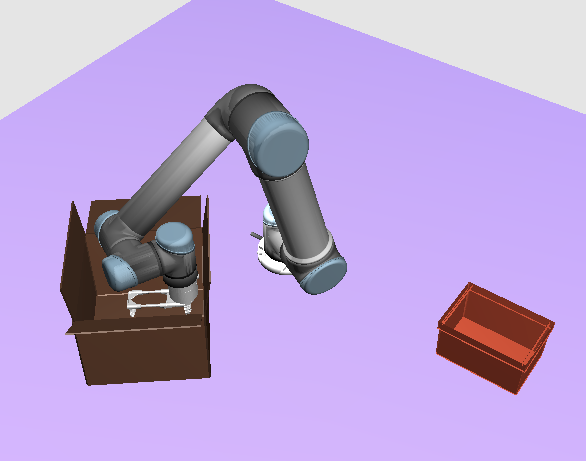
\includegraphics[width=5.8cm,height=4.7cm]{fiad_qfinal.png}\\
	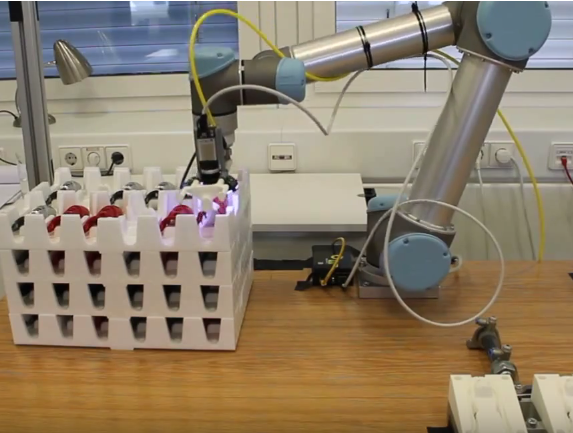
\includegraphics[width=5.8cm,height=4.7cm]{fiad_real.png}
	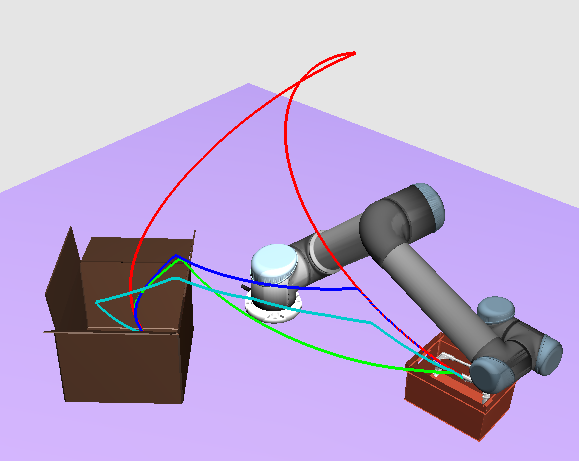
\includegraphics[width=5.8cm,height=4.7cm]{fiad_traj_prune.png}
	\caption{(Bottom left) An industrial use-case example proposed by Philips for 	
	the Factory-in-a-Day project~\cite{factory-day-video}. A similar environment 	
	has been created (top) to illustrate that our method can comply with an 
	industrial problem, where initial and final configurations of the UR5 are 
	constrained in boxes. End-effector trajectories 
	are illustrated (bottom right): initial (RRT-connect) in red, a RS 
	optimization in blue, a PRS one in cyan and the GB optimization in green.}
	\label{fiad}
\end{figure}

% UR5-spheres and fiad:
Some problems are 
involving a 6-axis manipulator arm, also called UR5, equipped with a bar or a 
gripper.
In a relatively free environment represented in Figure~\ref{fig:trajectories:ur5}, 
results from our method and RS are similar. 
Note also that the end-effector trajectory is completely different from the initial 
one: the robot is easily passing between the spheres, keeping its end-effector 
above.
For an UR5 working in a cluttered environment inspired by an industrial issue 
Figure~\ref{fiad}, path optimization efficiently returns a shorter solution, close 
to the result of RS and to what can be observed in 
reality~\cite{factory-day-video}.

% baxter:
A problem involving a Baxter-like\footnote{A torso rotation was added and 
the grippers were removed.} robot 
manipulating in an office environment is presented in
Figure~\ref{fig:trajectoriesbis:baxter}. The robot starts with its end-effectors 
above the computer and has to 
turn and reach the shelf. According to the left-hand trajectories quality (see the 
video for the full motion) and path lengths, the GB optimizer provides 
the smoothest motion.

\vspace{0.4cm}

In the three following high-DOF examples involving the PR2 robot, note that 
results are better in terms of path quality, as a result of the parasite 
DOF motions removal.

\begin{figure}
	\centering
	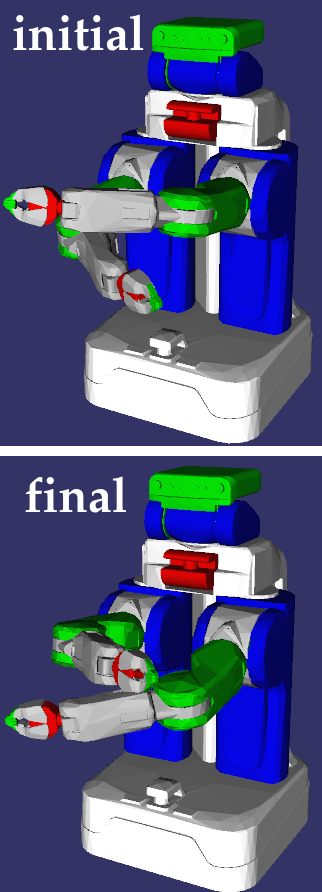
\includegraphics[height=4.9cm,width=1.8cm]{pr2_initial_final_vertical.png}
	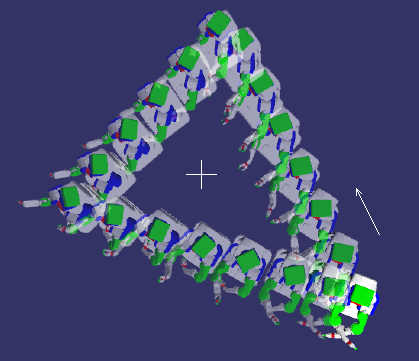
\includegraphics[width=5.7cm]{p0_pr2_alone_merged3.png}
	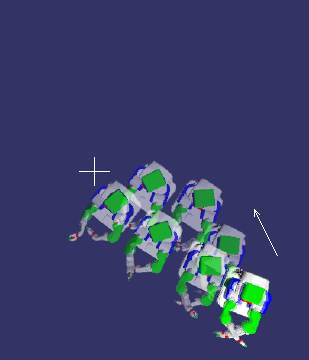
\includegraphics[height=4.9cm]{p1RS_pr2_alone_merged3.png}
	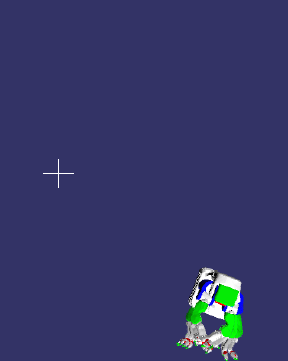
\includegraphics[height=4.9cm]{p1GB_pr2_alone_merged3.png}\\
	\caption{PR2-crossing-arms example. In this motion planning problem, PR2 robot 
	has just to 
exchange the positions of its arms. The task is simple, however, in absence of 
explicit indication, any probabilistic motion planner will compute a path that 
makes the PR2 mobile base purposelessly moving. This is the result of RRT-connect 
algorithm (left). Path optimization is expected to remove unnecessary motions. 
The popular RS algorithm fails in this case (middle). Our GB algorithm 
succeeds (right).}
	\label{pr2_final}
\end{figure}

% analysis PR2 alone:
In the example shown Figure~\ref{pr2_final} and in the video, the mobile 
40-DOF PR2 simply has to cross its arms from 
the left arm up position to the right arm up one, without any assumption about the group of DOF to activate (i.e. no DOF is locked). 
The RRT-connect planner 
returns detours and activates non-useful DOF such as the head, the torso lift 
and the translation on the ground. Such behavior induces a high initial path length. RS hardly optimizes the mobile base 
translation (Figure~\ref{pr2_final} middle) of the robot and other unnecessary DOF 
uses. Whereas the GB optimized-path mainly 
results in moving the arms as expected (Figure~\ref{pr2_final} right), just creating two collision-constraints between the arms. 
\textcolor{blue}{
In the PRS result, only presented in the video, the motion is less optimized than with RS: the arms are moving widely and the mobile base remains activated. One solution to remove such unnecessary DOF activation can be to try applying a partial shortcut on each DOF between the initial and final configuration. It appears that this step is more costly in terms of computation time than the GB duration, therefore it cannot be afforded by our PRS implementation. However, it could be applied as a preliminary optimization for each optimizer.
}

% analysis PR2 in kitchen:
Similar results are obtained on the PR2 performing manipulation tasks 
in a kitchen environment.
Firstly, the robot moves its hands from the top to the bottom of a table.
The different trajectories of the right gripper are indicated in Figure~\ref{fig:trajectoriesbis:kitchen1}.
Our optimizer manages to reduce the initial path length from visibility-PRM 
and improves the path quality 
just adding constraints between the table and the 
robot's arms. Thus, the robot just slightly moves 
backward and uses its arms DOF to avoid the table, instead of 
processing a large motion to get away from the table.
Secondly, another example of PR2 going from the set to the fridge 
door is presented Figure~\ref{fig:trajectoriesbis:kitchen2} with the mobile base
trajectories. Here, GB and RS results are similar in terms of length and rendering.

\vspace{0.3cm}

\begin{table}
\renewcommand{\arraystretch}{1.3}
\centering
\scalebox{0.9}{
  \begin{tabular}{cccC{1.3cm}C{1.3cm}C{1.3cm}}
  \toprule
  \multirow{2}{*}{\textbf{Problem}} &  & \multirow{2}{*}{Computation time} & \multicolumn{3}{c}{\minibox{Relative remaining length (\%)}} \\
   & & &  GB  &  RS  &  PRS  \\
  \midrule
  \midrule
  %\textbf{2D slidding-robot (Fig.~\ref{2D_long} right)} & & 11.9 ms & 78.3 & 68.0 & 81.8 \\
  \textbf{Freeflyer-puzzle} & \todo ($\alpha_{init}=0.1$) & 0 ms & 0 & 0 & 0 \\
  \textbf{Double-arm 4-DOF} & & 39.6 ms & 46.8 & 55.5 & 63.5 \\
  \textbf{UR5-with-spheres} & (RRT, $\alpha_{init}=0.3$) & 3.18 s & 53.8 & 47.5 & 67.8 \\
  \textbf{UR5-industrial-example} & \todo (RRT) & 5.50 s & 55.2 & 41.9 & 65.1 \\
  \textbf{Baxter-in-office} & \todo & 125 s & 26.0 & 36.8 & 74.7 \\
  \textbf{PR2-crossing-arms} & & 882 ms & 19.9 & 43.2 & 95.2 \\
  \textbf{PR2-in-kitchen-1} & \todo & 12.8 s & 30.6 & 45.3 & 90.9 \\
  \bottomrule
  \end{tabular}  }%scalebox
\caption{\textcolor{blue}{Average results for 50 runs of several examples presented in the 
paper. For each run, a solution path is planned by Visibility-PRM 
(unless `RRT' for RRT-connect is mentioned) as initial guess for the 
three optimizers. The RS and PRS results correspond to averages of 50 
launches of the random optimizers on each initial guess. The GB 
computation time is the work duration allowed for the random optimizers. 
$\alpha_{init}=0.2$ unless another value is specified.
%For the PR2-crossing-arms example only, the right column represents the distance that is traveled by the robot mobile base during the different paths.
}}
\label{tab:results}
\end{table}

% convergence graphs:
\textcolor{blue}{
For some of the presented benchmarks, convergence graphs of the path 
length reduction are 
given Figure~\ref{fig:remainingLength}. The chosen initial paths are unchanged, 
e.g. correspond to Figures~\ref{fig:trajectories} and~\ref{fig:trajectoriesbis}. 
Each graph illustrates the percent ratio of the optimized path length over the initial path length, during the optimization time.
For the random optimizers curves, averages and standard deviations on 50 
launches are given. It is not a surprise that GB is globally slower than RS due to the difference of the computations complexity during the optimization. Thus RS converges faster. However, it seems that GB catches up and overcomes RS before ending (see Figures~\ref{fig:remainingLengthComp:pr2alone} and~\ref{fig:remainingLengthComp:pr2kitchen1}), thanks to the optimization of the mobile base motion. Therefore, it could be interesting to investigate the performance of a composed optimizer, starting by a RS stage until convergence and finishing by a GB stage to improve the path length reduction.
As previously stated in the freeflyer-example (see Figures~\ref{fig:trajectories:puzzle} and~\ref{fig:remainingLengthComp:puzzle}), GB is not only less efficient than RS and PRS but converges slower. 
This can be partly explained by the fact that collision checking is rapidly performed in such basic geometry problem. This favors the random shortcut tries while GB spends time on the LCQP resolution.
}

\vspace{0.3cm}

\textcolor{blue}{
Since the GB optimizer results depend on the shape of the initial guess, e.g. the number of waypoints and the proximity to obstacles, results averages for 50 initial paths of each benchmark are presented in Table~\ref{tab:results}. As mentioned, the paths are obtained from Visibility-PRM or RRT-connect. Due to their nature, these motion planners provide different types of path: the output of Visibility-PRM contains less waypoints and does not tend to be close to the contact, behavior induced by the extension process of RRT.
}
In some cases, $\alpha_{init}$ was 
reduced to comply with very narrow passages, or increased in the opposite case.
\textcolor{blue}{
The following section deals with the $\alpha_{init}$ influence in depth.
}

\textcolor{blue}{
The results seems to be consistent with the trajectories analysis and convergence graphs. Except the low-DOF problem of the puzzle, our method provides 
shorter or similar results compared to RS. Results seems even to be better when the number of DOF increase, as the baxter and PR2 examples.
Note that the path length does not necessary account for the parasite motions disappearance.
}
%Finally, the complete vanishing of the mobile base motion in the GB optimized path is noted. Thus the issue addressed in Figure~\ref{decoupled_DOF_optimization} is solved considering this DOF.


\subsubsection{Analysis of $\alpha_{init}$ influence}

\begin{figure}
	\centering
	\subfigure[2D slidding-robot (Fig.~\ref{2D_long} right)]{
		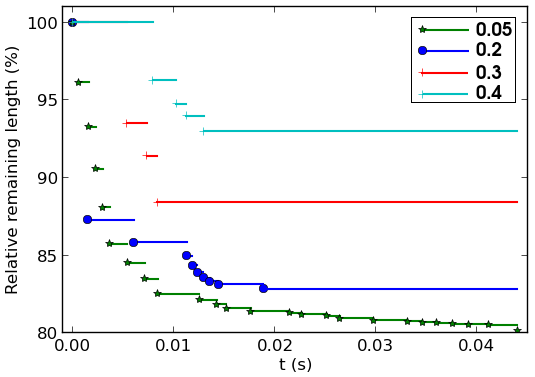
\includegraphics[width=6.8cm,height=5.5cm]{potential2D_alphaInit.png}
		\label{fig:remainingLengthAlphaInit:2Drobot}
	}
	\subfigure[Double-arm]{
		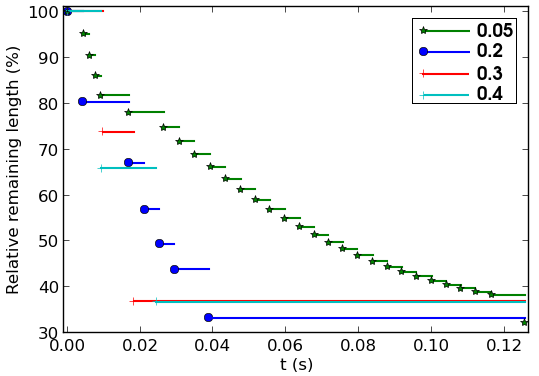
\includegraphics[width=6.8cm,height=5.5cm]{ur2_alphaInit.png}
		\label{fig:remainingLengthAlphaInit:double_arm}
	}
  	\subfigure[Freeflyer-puzzle]{
		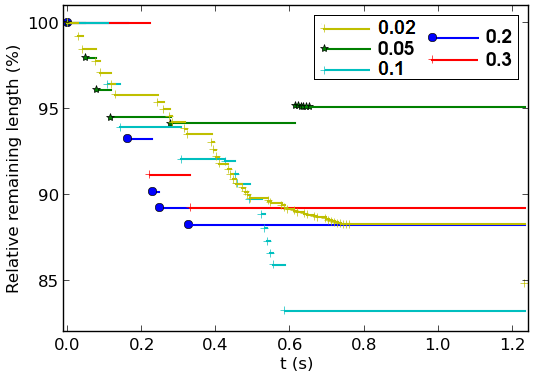
\includegraphics[width=6.8cm,height=5.5cm]{puzzle_alphaInit.png}
		\label{fig:remainingLengthAlphaInit:puzzle}
	}
	\subfigure[Baxter-in-office]{
		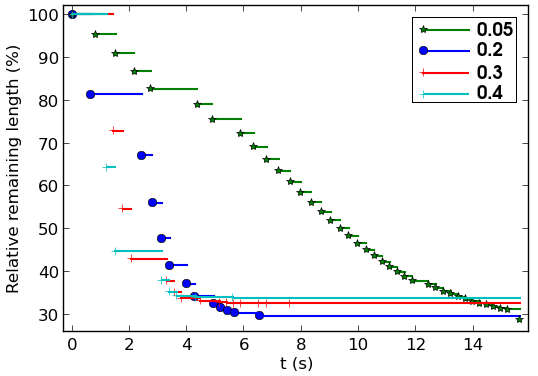
\includegraphics[width=6.8cm,height=5.5cm]{baxter_alphaInit.png}
		\label{fig:remainingLengthAlphaInit:baxter}
	}
  \caption{\textcolor{blue}{Influence of $\alpha_{init}$ on the convergence graphs of the GB optimizer. For each benchmark, the considered intial paths correspond to the ones of Figures~\ref{fig:trajectories} and~\ref{fig:trajectoriesbis}.}}
  \label{fig:remainingLengthAlphaInit}
\end{figure}

\textcolor{blue}{
This section deals with the influence of the parameter $\alpha_{init}$ on the 
GB convergence. Reducing $\alpha_{init}$ makes Algorithm~\ref{algo:gradient} 
process smaller iterations. Some expected behaviors are visible in 
Figure~\ref{fig:remainingLengthAlphaInit}. 
For instance, Figure~\ref{fig:remainingLengthAlphaInit:2Drobot} illustrates an 
expected influence of a $\alpha_{init}$ reduction on the final path lengths. Besides, commonly to Figures~\ref{fig:remainingLengthAlphaInit:2Drobot}
,~\ref{fig:remainingLengthAlphaInit:double_arm} 
and~\ref{fig:remainingLengthAlphaInit:baxter}, $\alpha_{init}=0.05$ has the higher convergence time.
}

\textcolor{blue}{
However, due to the strong non-linearity of the constraints, reduced iterations 
do not necessary lead to a slower but refined solution. GB can stops earlier 
in local minimum, which may also have a better path length reduction. This is 
the case of Figure~\ref{fig:remainingLengthAlphaInit:double_arm} where $\alpha_{init}=0.2$ results in a shorter path than $\alpha_{init}=0.05$. More surprisingly in Figure~\ref{fig:remainingLengthAlphaInit:double_arm}, $\alpha_{init}=0.05$ leads to the worse reduction.
}

\textcolor{blue}{
Instead of investigating a way to find a $\alpha_{init}$ conditioned by the problem and the initial path, we plan to adapt $\alpha$ from Algorithm~\ref{algo:gradient} due to geometrical considerations, as the continuous collision checker.
}

\subsubsection{Influence of a pruning preliminary step}
\textcolor{blue}{For the ur5-industrial benchmark, we compared the optimization convergence graphs with and without a pruning step. Prune was implemented following~\cite{GeraertsIJRR07}, to remove redundant nodes in the initial path by creating valid shortcuts between the waypoints. RRT-connect has been chosen as motion planner because it usually produces more waypoints that Visibility-PRM, so the impact of pruning is more accountable. Results are given Figure~\ref{fig:pruningInfluence}. The path length reduction of the three optimizers are still compared, but the notable information is the computation time of GB that is 16 times higher without pruning. Such lower computation time prevents the random optimizers to converge, so the GB result appears as better.
}

\textcolor{blue}{Note that, if applying Prune always reduces the GB optimization time, it sometimes spoils the path length reduction. In fact, there can be cases where multiple waypoints are useful to bypass an obstacle, rather than a long straight line in the configuration space.
}

\begin{figure}[H]
	\centering
	\subfigure[Without pruning]{
		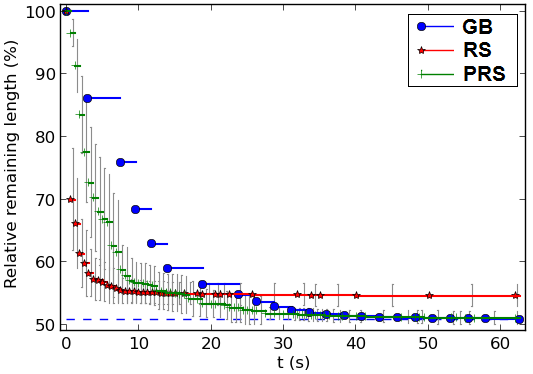
\includegraphics[width=6.8cm,height=5.5cm]{fiadRRT_comp.png}
		\label{fig:pruningInfluence:comp}
	}
	\subfigure[With pruning]{
		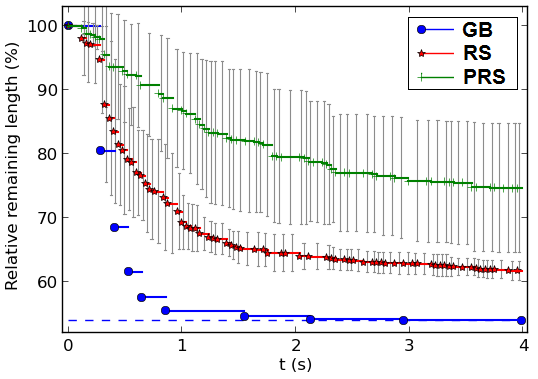
\includegraphics[width=6.8cm,height=5.5cm]{fiadRRT_comp_prune.png}
		\label{fig:pruningInfluence:comp_prune}
	}
  \caption{\textcolor{blue}{Influence of a pruning step on the optimization processes. RRT-connect provides an initial path with 62 waypoints, which is downed to two waypoints by Prune. Concerning the path length, it is only reduced of 6.2\% by Prune. Thus, final path lengths provided by GB in both cases are equivalent, the major difference results in the computation time of GB.}}
  \label{fig:pruningInfluence}
\end{figure}


\section{CONCLUSIONS}
We managed to settle a path optimization for navigation and manipulation problems, and tested it with various robots and environments. Our algorithm uses standard 
numerical tools as collision checking, linearized one-dimensional constraint
and \textcolor{blue}{LC}QP resolution. It correlates them in a 
simple but effective way, and the algorithm structure is organized so that its 
convergence is guaranteed. Furthermore, 
our method only requires collision checking, therefore neither 
geometry pre-processing nor 
offline optimization are necessary to remain time-competitive. We demonstrate 
that the optimizer may be 
time-competitive compared to random shortcut in complex models where collision tests 
are time-consuming. 
It also proposes better quality paths, reducing the path length and removing 
unnecessary DOF motions. 
Finally, our optimizer manages to reduce a local detour in a long path while random 
shortcut methods will mostly fail.

For future work, we have room for improvement. We can take advantage of the sparsity of 
the constraint Jacobian to reduce computation time. We may also adapt the iteration 
scalar parameter from geometries considerations on the current path, e.g. using a lower 
bound of the distance between nearest objects, since this bound can be returned by 
the collision checker.

\section*{Funding}
This work has been supported by the project ERC Advanced Grant 340050 Actanthrope and by the FP~7 project Factory in a Day under grant agreement n°~609206.

\begin{figure}
	\centering
	\subfigure[Double-arm]{
		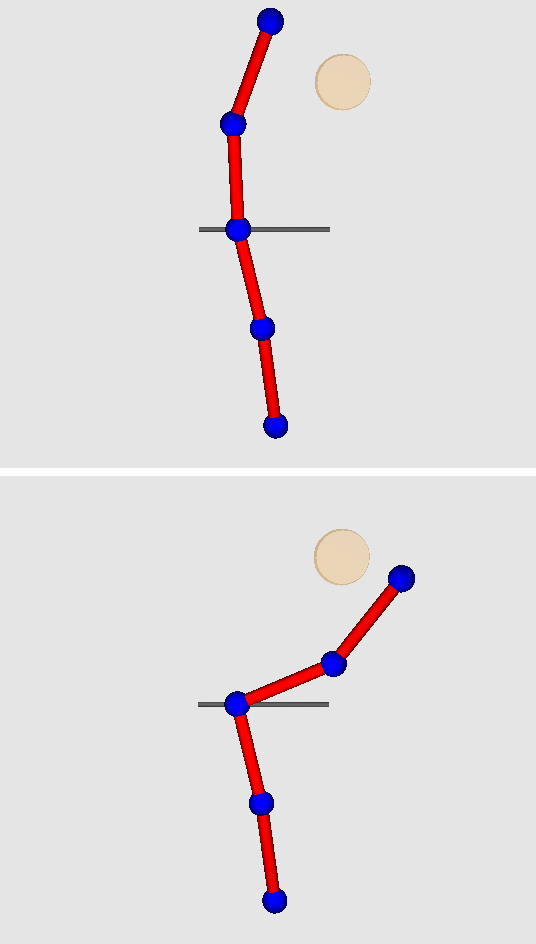
\includegraphics[width=2.9cm,height=5.5cm]{ur2_initfinal.png}
		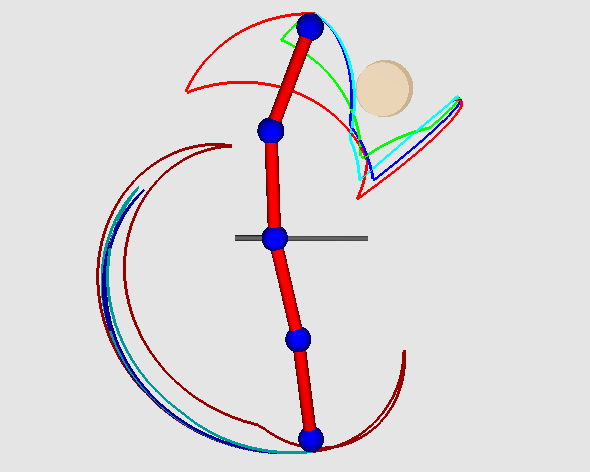
\includegraphics[width=6.5cm,height=5.5cm]{ur2_traj.png}
		\label{fig:trajectories:double_arm}
	}
	\subfigure[Freeflyer-puzzle]{
		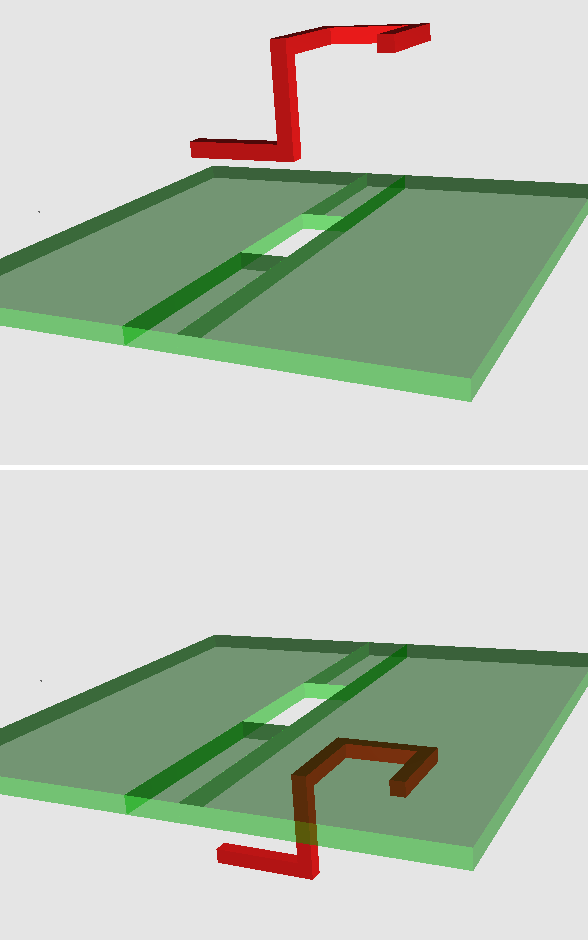
\includegraphics[width=2.9cm,height=5.5cm]{puzzle_initfinal.png}
		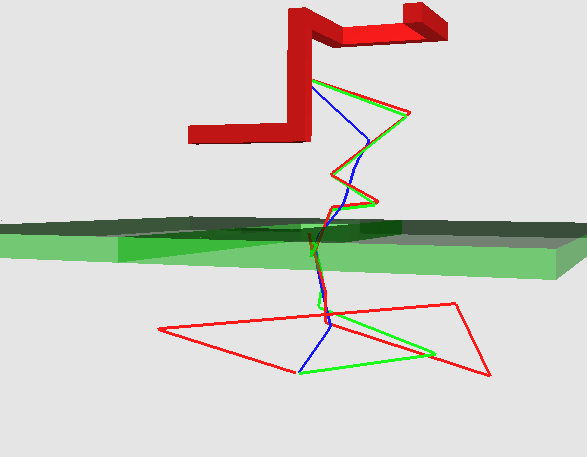
\includegraphics[width=6.5cm,height=5.5cm]{puzzle_traj.png}
		\label{fig:trajectories:puzzle}
	}
	\subfigure[UR5-with-spheres]{
		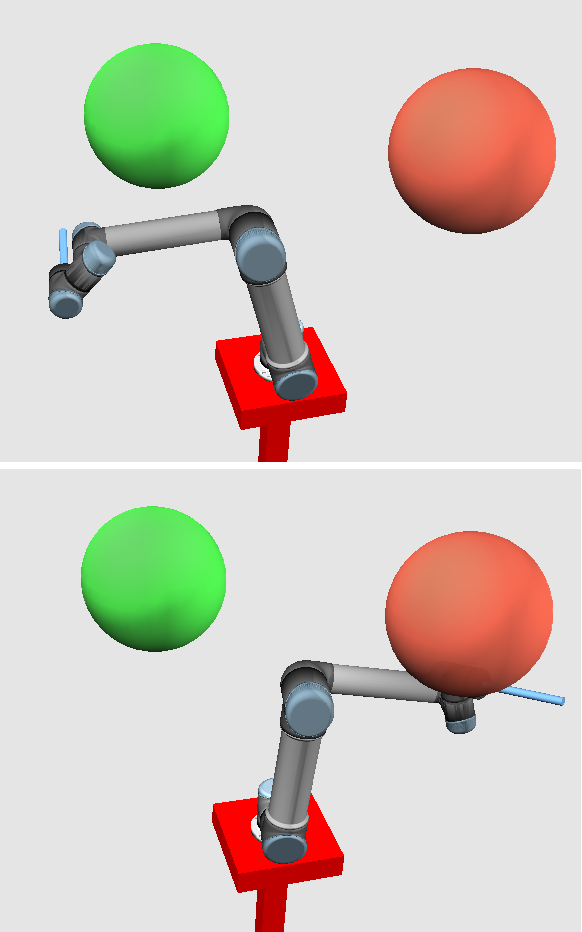
\includegraphics[width=2.9cm,height=5.5cm]{ur5spheres_initfinal.png}
		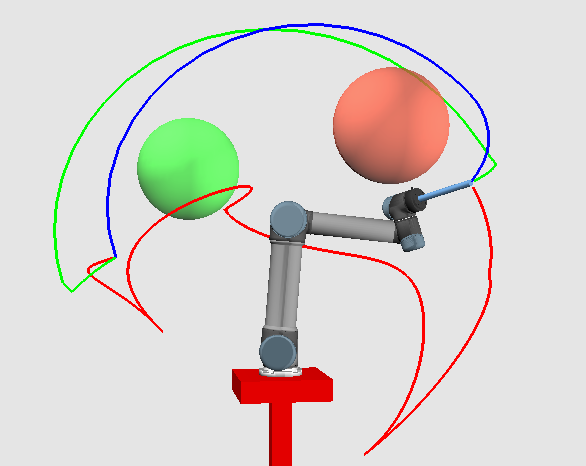
\includegraphics[width=6.5cm,height=5.5cm]{ur5spheres_traj.png}
		\label{fig:trajectories:ur5}
	}
  \caption{(Left) Initial and final configurations.
  (Right) Trajectories of end-effectors or centers along the 
  different paths: the initial path is represented in red, the RS 
  output in blue, the PRS output in cyan (top only) and the GB optimized path 
  in green. The full robots 
  motions can also be visualized in the joined video. The 
  trajectories comparison highlights the optimization success of our method, 
  which manages to deliver a shorter or similar path compared to the RS output. 
  GB also cancels unecessary DOF activation contrary to RS and PRS (see the 
  lower arm in top-right Figure).}
  \label{fig:trajectories}
\end{figure}

\begin{figure}
	\centering
	\subfigure[PR2-in-kitchen-1]{
		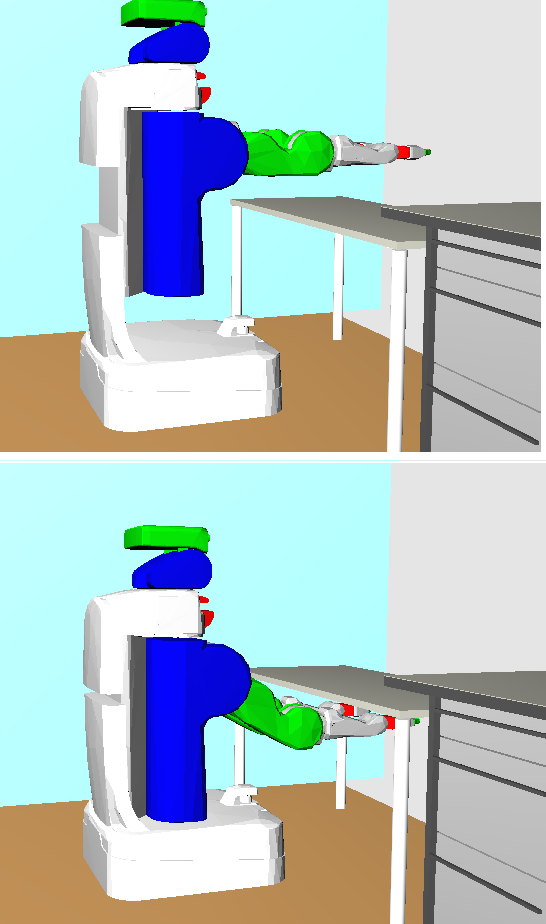
\includegraphics[width=2.9cm,height=5.5cm]{pr2kitchen1_initfinal.png}
		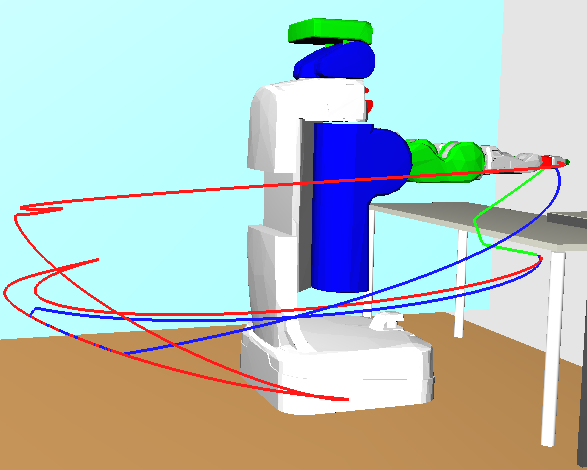
\includegraphics[width=6.5cm,height=5.5cm]{pr2kitchen1_traj.png}
		\label{fig:trajectoriesbis:kitchen1}
	}
	\subfigure[PR2-in-kitchen-2]{
		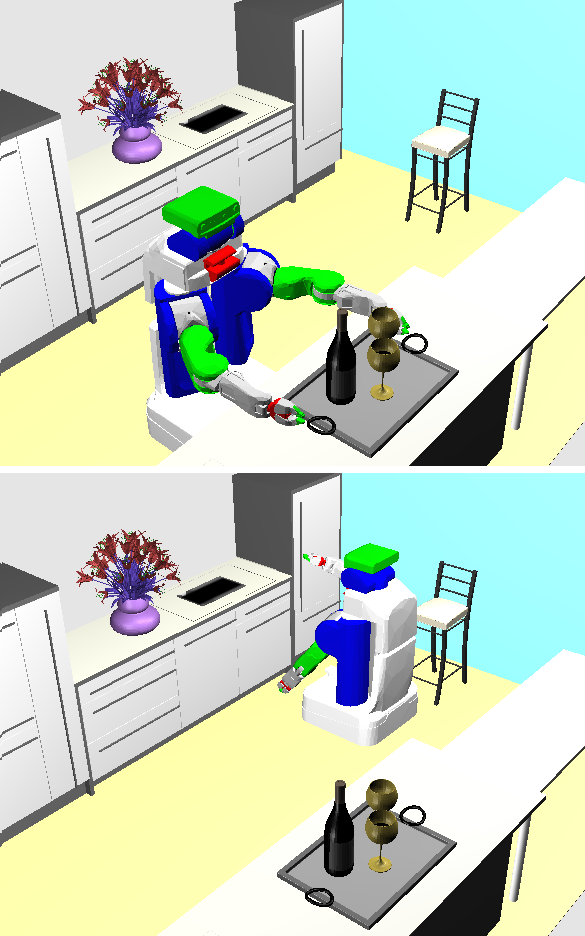
\includegraphics[width=2.9cm,height=5.5cm]{pr2kitchen2_initfinal.png}
		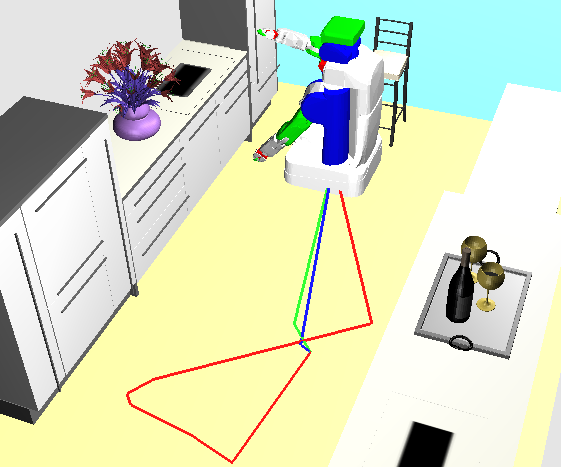
\includegraphics[width=6.5cm,height=5.5cm]{pr2kitchen2_traj.png}
		\label{fig:trajectoriesbis:kitchen2}
	}
	\subfigure[Baxter-in-office]{
		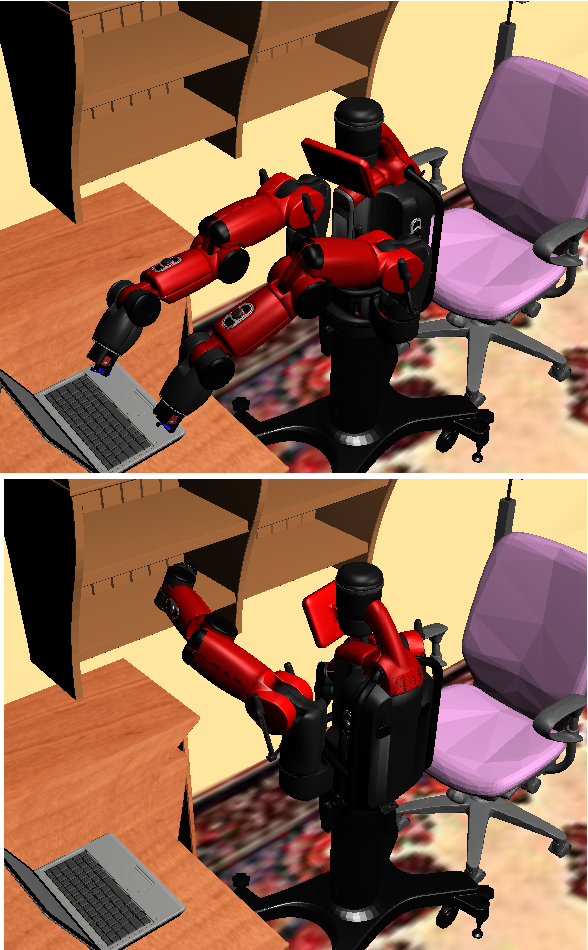
\includegraphics[width=2.9cm,height=5.5cm]{baxter_initfinal.png}
		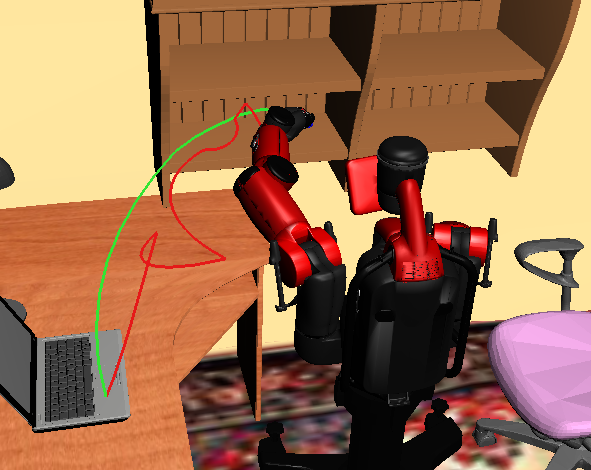
\includegraphics[width=6.5cm,height=5.5cm]{baxter_traj.png}
		\label{fig:trajectoriesbis:baxter}
	}
  \caption{Other trajectories comparisons of end-effectors or mobile bases (initial path in red, RS output in blue, PRS output in cyan and GB output in green).}
  \label{fig:trajectoriesbis}
\end{figure}

\begin{figure}
	\centering
	\subfigure[2D sliding robot (Fig.~\ref{2D_long})]{
		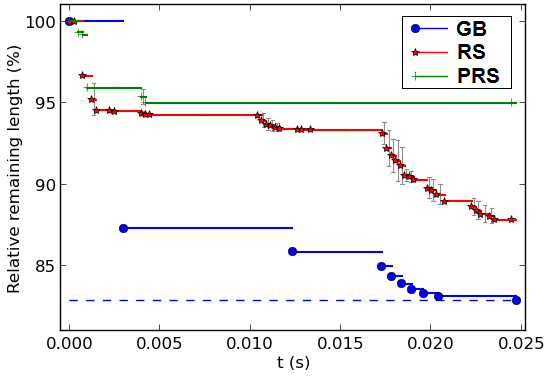
\includegraphics[width=6.5cm,height=5.5cm]{potential2D_comp.png}
		\label{fig:remainingLengthComp:potential2D}
	}
	\subfigure[Freeflyer-puzzle]{
		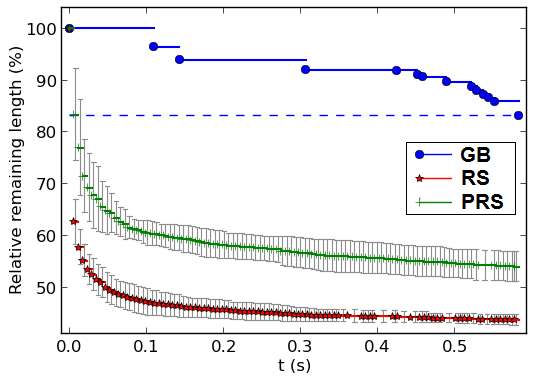
\includegraphics[width=6.5cm,height=5.5cm]{puzzle_comp.png}
		\label{fig:remainingLengthComp:puzzle}
	}
	\subfigure[UR5-with-spheres]{
		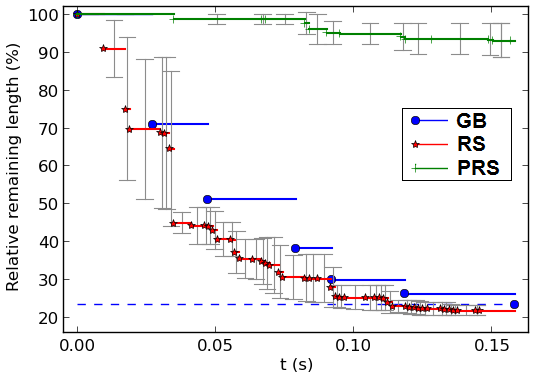
\includegraphics[width=6.5cm,height=5.5cm]{ur5spheres_comp.png}
		\label{fig:remainingLengthComp:ur5sphere}
	}
	\subfigure[PR2-crossing-arms]{
		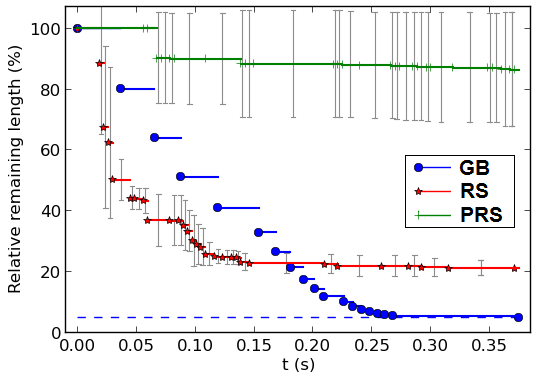
\includegraphics[width=6.5cm,height=5.5cm]{pr2crossing_comp_prune.png}
		\label{fig:remainingLengthComp:pr2alone}
	}
	\subfigure[PR2-in-kitchen-1]{
		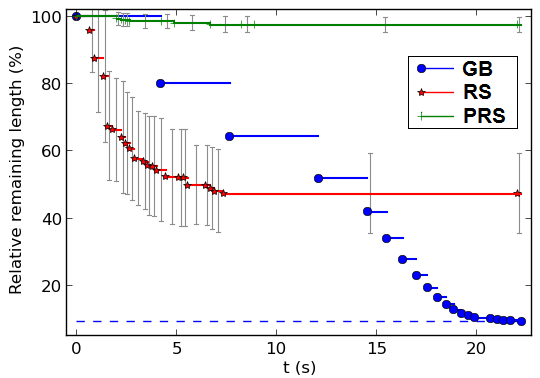
\includegraphics[width=6.5cm,height=5.5cm]{pr2kitchen1_comp.png}
		\label{fig:remainingLengthComp:pr2kitchen1}
	}
	\subfigure[Baxter-in-office]{
		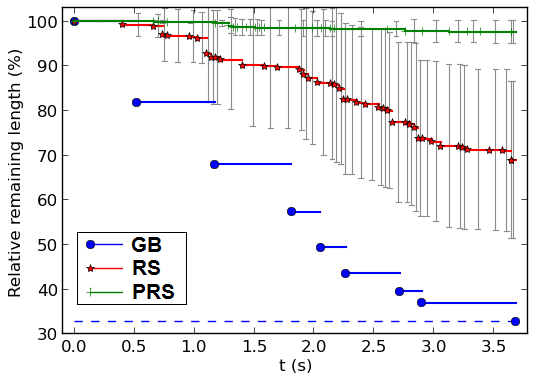
\includegraphics[width=6.5cm,height=5.5cm]{baxter_comp_prune.png}
		\label{fig:remainingLengthComp:baxter}
	}
  \caption{\textcolor{blue}{Convergence graphs of the three optimizers during the optimization process. For each benchmark, the considered intial paths correspond to the ones of Figures~\ref{fig:trajectories} and~\ref{fig:trajectoriesbis}. The remaining path length relative to the initial one is represented. The dashed blue line is the final result of GB. For RS and PRS, the averages and standard deviations (in grey) over 50 launches are plotted.}}
  \label{fig:remainingLength}
\end{figure}


\bibliographystyle{tADR}
\bibliography{paper}

\end{document}
